%\documentclass[11pt]{book}
\documentclass[usletter]{book}
\usepackage{graphicx}
\usepackage{amssymb}

\textwidth = 6.5 in
\textheight = 8 in
\oddsidemargin = 0.0 in
\evensidemargin = 0.0 in
\topmargin = 0.0 in
\headheight = 0.0 in
\headsep = 0.5 in
\parskip = 0.2in
\parindent = 0.0in


\title{User's Manual \\ OpenBTS\textsuperscript{\scriptsize \textregistered} Release 2.6 Series Software}
\author{Copyright 2010, Kestrel Signal Processing, Inc.\\ All rights reserved; do not redistribute.}

\begin{document}
\maketitle

\tableofcontents
\listoffigures

\chapter{Introduction}
OpenBTS 2.6 was first deployed in a pilot network with Telecom Niue in March 2010.  It was released publicly in June 2010.

\section{Scope and Audience}
This document describes the organization and operation of the OpenBTS 2.6-series GSM access point software.  It is intended for use by software developers and network operators.

\section{Disclaimers}

\subsection{Warranty}
The OpenBTS software and its associated documentation are provided with NO WARRANTY OF ANY KIND.  However, Kestrel Signal Processing, Inc.\ welcomes any reports of software failures or documentation errors.
Annual maintenance and support contracts are available from Kestrel Signal Processing.

This manual is a description of the OpenBTS 2.6 software, not a specification.
In any discrepancy between the software and this manual, the software source code is authoritative.

\subsection{Patent Laws}
The use of this software to provide GSM services may result in the use of
patented technologies.  The user of this software is required to take whatever
actions are necessary to avoid patent infringement.

\subsection{Trademarks}
``OpenBTS'' is a registered trademark of Kestrel Signal Processing, Inc. (KSP), a
California corporation.  KSP reserves the right to control the use of this
trademark.  Do not use this trademark in commerce without permission and do not
rebrand OpenBTS under a different trademark.

``Asterisk'' is a trademark of Digium, Inc.

\subsection{Telecom and Radio Spectrum Laws}
The primary function of the OpenBTS software is the provision of telecommunications service
over a radio link.  This activity is heavily regulated nearly everywhere in
the world.  Users of this software are expected to comply with local, national and international
regulations in the jurisdictions where this sortware is used with radio equipment.

\subsection{Software Licensing and Distribution}
A subset of the OpenBTS source code, including all of OpenBTS release 2.6, is distributed publicly under GPLv3 and AGPLv3. KSP reserves the right to distribute any or all of the OpenBTS source code, with the exception of 3rd-party GPL components, under other licenses. KSP reserves the right to withhold any or all of the source code from future public releases.



\section{Abbreviations}
\begin{itemize}
	\item ARFCN -- absolute radio frequency channel number
	\item BTS -- base transceiver subsystem
	\item dBm -- decibel milliwatts
	\item FEC -- forward error correction
	\item kHz -- kilohertz
	\item KSP -- Kestrel Signal Processing, Inc.
	\item LNA -- low-noise amplifier
	\item PA -- power amplifier
	\item preamp -- low-noise amplifier
	\item RF -- radio frequency
	\item TDM -- time-domain multiplexing
	\item VDC -- Volts, direct current
	\item W -- Watts
\end{itemize}


\section{References}

\subsection{ETSI/3GPP}
This document references the following GSM specifications, which can be downloaded for free from \\

http://webapp.etsi.org/key/queryform.asp \\

\begin{itemize}
	\item GSM 04.06: ``Digital cellular telecommunications system (Phase 2+);  Mobile Station - Base Station System (MS - BSS) interface;  Data Link (DL) layer specification''
	\item GSM 04.08: ``Digital cellular telecommunications system (Phase 2+); Mobile radio interface layer 3 specification''
	\item GSM 05.02: ``Digital cellular telecommunications system (Phase 2+);  Multiplexing and multiple access on the radio path''
	\item GSM 05.03: ``Digital cellular telecommunications system (Phase 2+);  Channel coding''
	\item GSM 05.05: ``Digital cellular telecommunications system (Phase 2+); Radio transmission and reception''
	\item GSM 05.08: ``Digital cellular telecommunications system (Phase 2+); Radio subsystem link control"
	\item GSM 05.10: ``Digital cellular telecommunications system (Phase 2+); Radio subsystem synchronization''
\end{itemize}

\subsection{Unix Documentation}
This document references manual pages for the following Linux/Unix utilities:
\begin{itemize}
	\item screen
\end{itemize}


\subsection{IETF}
This document references the following IETF standards, which can be downloaded for free from \\

http://tools.ietf.org/html/ \\

\begin{itemize}
	\item RFC-3428: ``Session Initiation Protocol (SIP) Extension for Instant Messaging''
\end{itemize}



\chapter{The OpenBTS Application Suite}
A complete OpenBTS 2.6 installation comprises four distinct applications:
\begin{itemize}
	\item {\bf OpenBTS} -- The actual OpenBTS application, containing most of the GSM stack above the radiomodem.
	\item {\bf Transceiver} -- The software radiomodem and hardware control interface.
	\item {\bf Asterisk} -- The VoIP PBX or ``softswitch''.
	\item {\bf Smqueue} -- The RFC-3428 store-and-forward server for text messaging.
\end{itemize}
The OpenBTS and Transceiver applications must run inside the BTS unit.  The Asterisk and Smqueue applications must run on the same computer, but that computer can be remote from the BTS unit.
The organization of these applications is shown in Figure~\ref{fig:suite}.

\begin{figure}[htbp]
\begin{center}
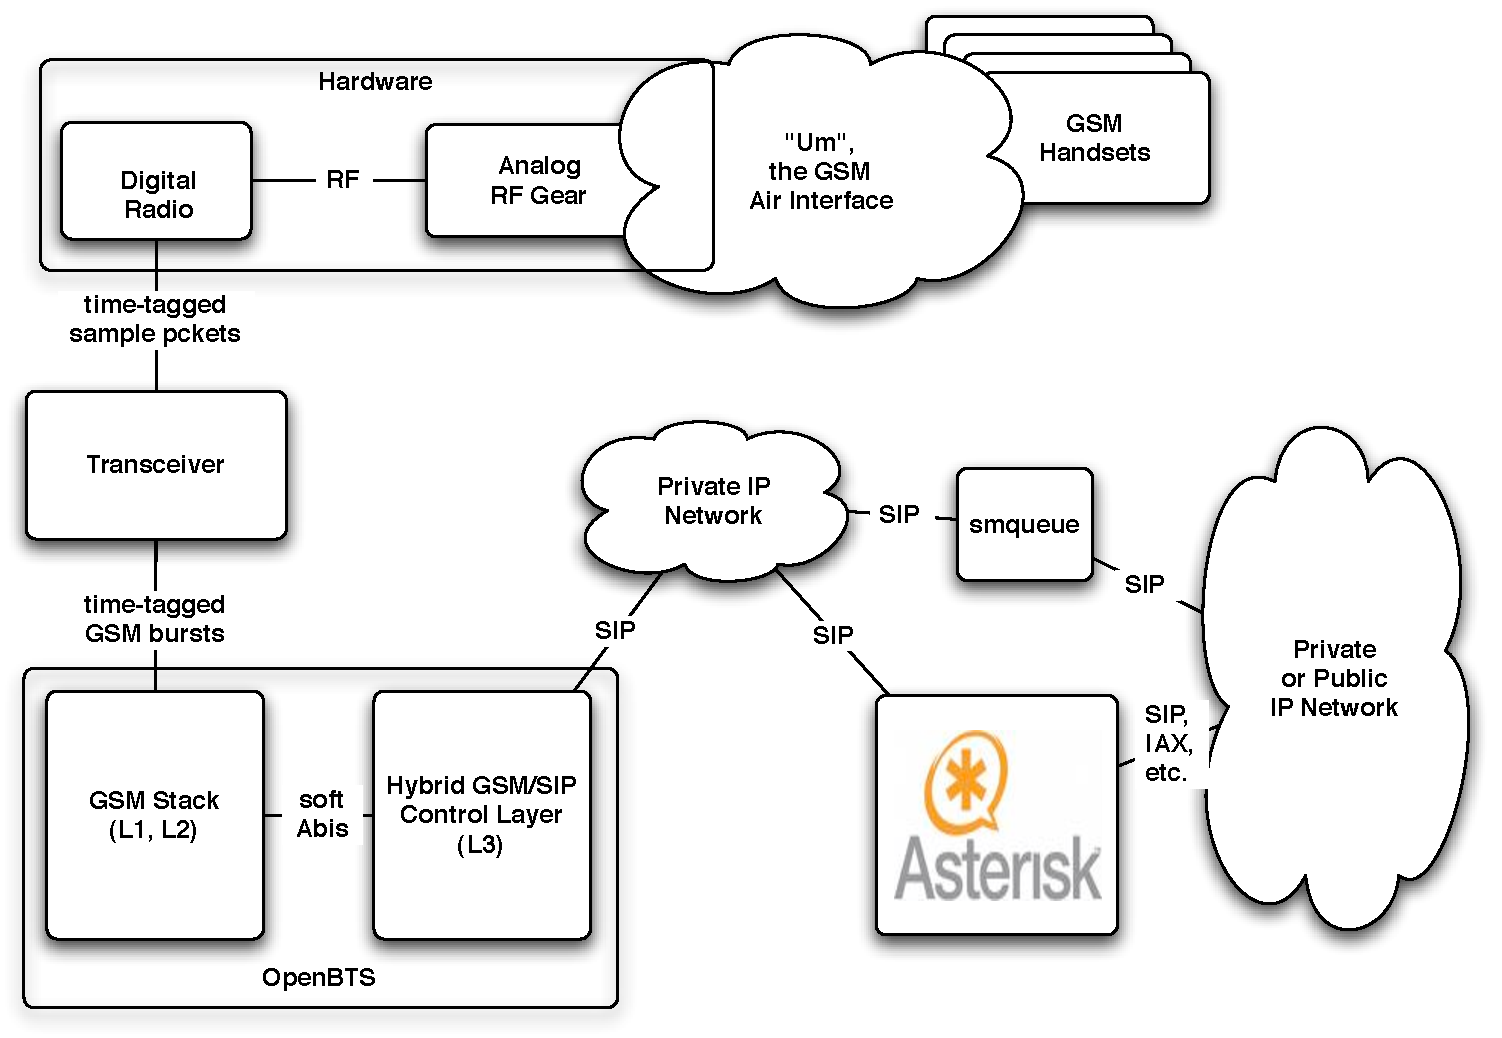
\includegraphics[width=6in]{OpenBTSArch.pdf}
\caption{Components of the OpenBTS application suite and their communication channels.}
\label{fig:suite}
\end{center}
\end{figure}



\section{OpenBTS}
The OpenBTS application contains:
\begin{itemize}
	\item L1 TDM functions (GSM 05.02)
	\item L1 FEC functions (GSM 05.03)
	\item L1 closed loop power and timing controls (GSM 05.08 and 05.10)
	\item L2 LAPDm (GSM 04.06)
	\item L3 radio resource management functions (GSM 04.08)
	\item L3 GSM-SIP gateway for mobility management
	\item L3 GSM-SIP gateway for call control
	\item L4 GSM-SIP gateway for text messaging
\end{itemize}
The general design approach of OpenBTS is not to implement any function above L3, so at L3 every subprotocol of GSM is either terminated locally or translated through a gateway to some other protocol for handling by an external application.  Similarly, OpenBTS itself does not contain any speech transcoding functions above the L1 FEC parts.

\section{Transceiver}
The transceiver application performs the radiomodem functions of GSM 05.05 and manages the USB interface to the radio hardware.  See Chapter~\ref{chap:transceiver} for more information.

\section{Asterisk}
OpenBTS uses Asterisk to perform the call control functions that would normally be performed by the mobile switching center in a conventional GSM network.  OpenBTS uses the Asterisk SIP registry as a substitute for the home location register found in a conventional GSM network.  OpenBTS also relies on Asterisk for any transcoding functions.  See Chapter~\ref{chap:Connecting} of this document for specific information about integration between OpenBTS and Asterisk.  For more information on Asterisk itself, a good resource is the book \underline{Asterisk: The Future of Telephony} by Jim Van Meggelen, Jared Smith, and Leif Madsen, from O'Reilly Publishing, ISBN 0-596-00962-3.  

OpenBTS has been used with VoIP PBX applications other than Asterisk, however KSP does not normally support those configurations.

\section{Smqueue}
Smqueue is an RFC-3428 store-and-forward server that is used for text messaging in the OpenBTS system.  Smqueue is required to send a text message from one handset to another, or to provide reliable delivery of text messages to a handset from any source.  See Chapter~\ref{chap:smqueue} for more information.

\section{The Restart Loop \& ``Screen''}
In embedded configurations used in KSP systems, OpenBTS starts during system initialization and is executed from a script called ``runloop.sh''.
The purpose of this script is to automatically restart OpenBTS and the transceiver process should either one crash or exit.
In Linux systems, this script is invoked as a detached session from /etc/rc.local with the Unix ``screen'' utility.
Please refer to the Unix manual page for ``screen'' for more information on the capabilities of the screen utility.



\chapter{The OpenBTS Air Interface}
\label{chap:Um}
This chapter describes the GSM air interface, ``Um'', as implemented by OpenBTS 2.6.
It is not really necessary to fully understand this chapter to use OpenBTS or even to develop new features for it, but the information is given here for completeness and to provide references to important parts of the GSM specifications to support more detailed study.

Broadly speaking, Um is organized into channels and layers, as shown in Figure~\ref{fig:GSMLayers}.
The rest of this chapter will explain this diagram.

\begin{figure}[htbp]
\begin{center}
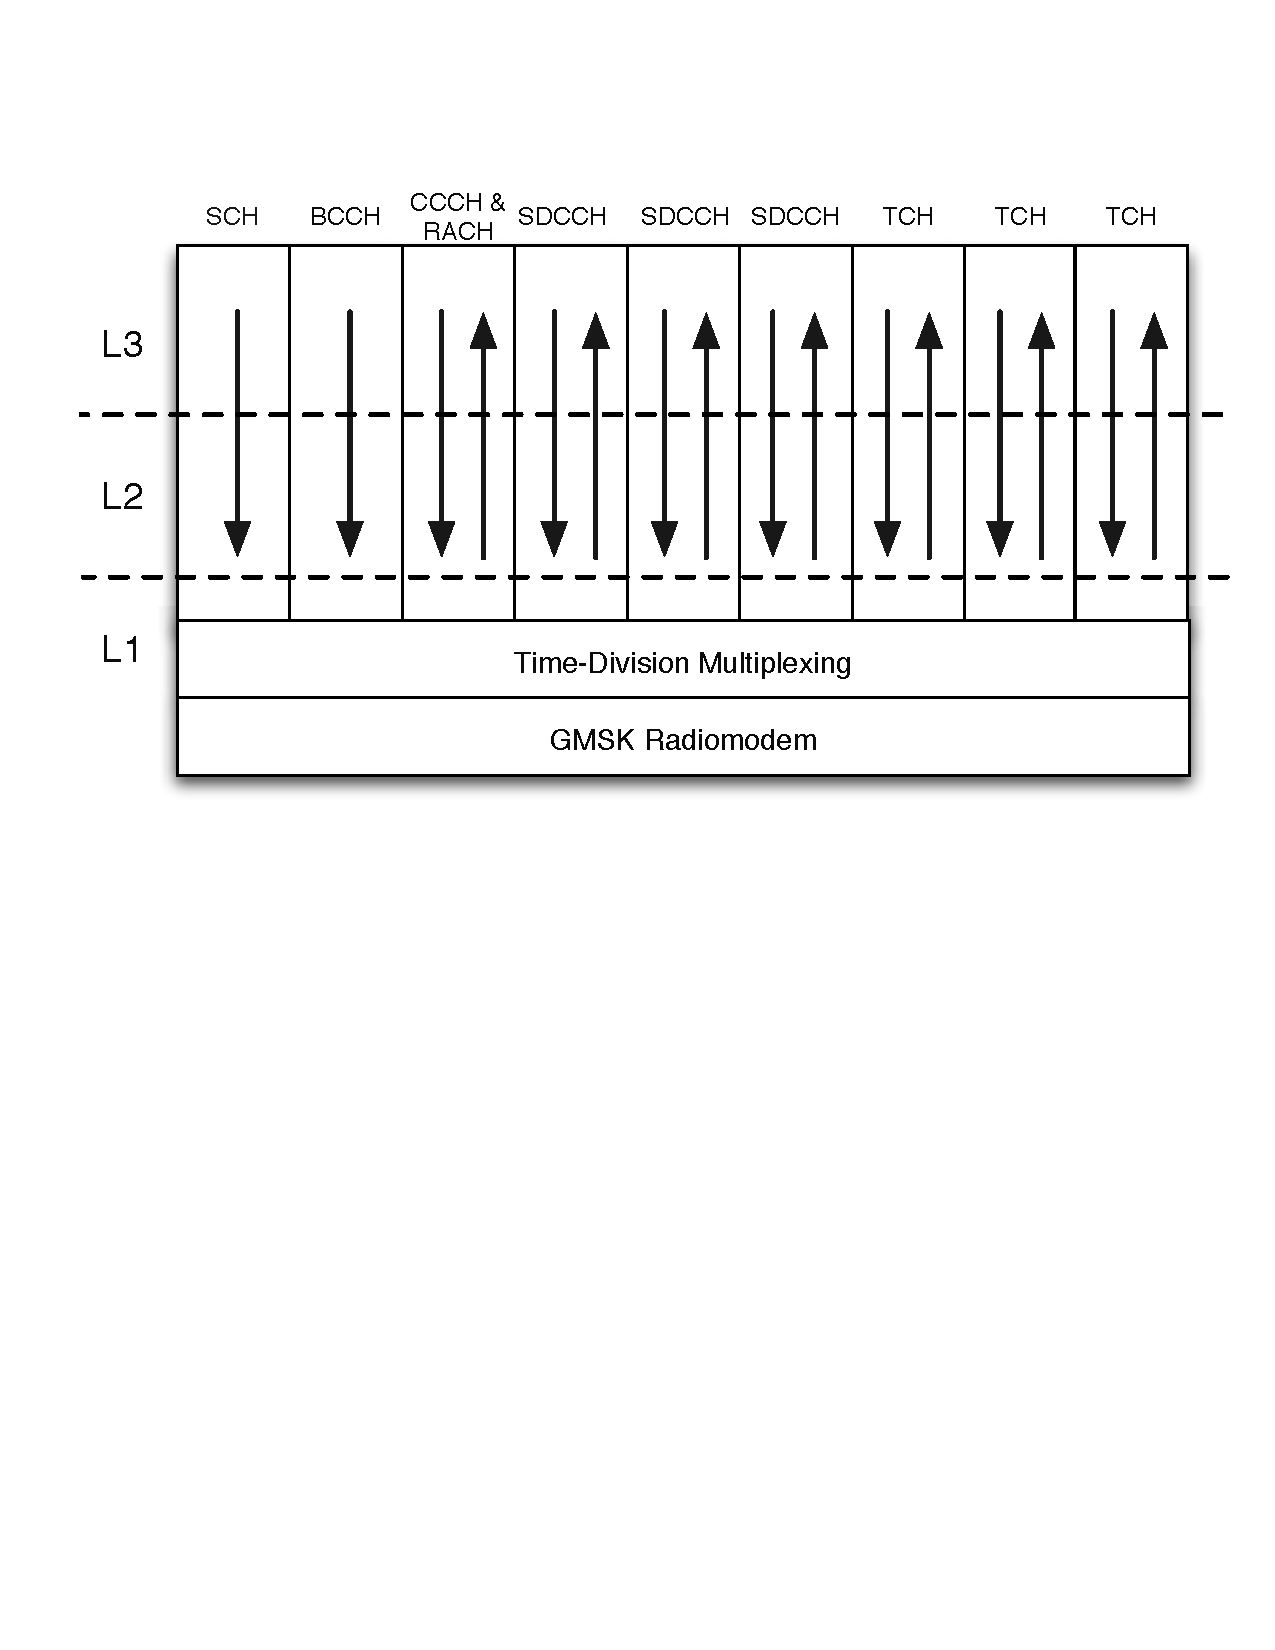
\includegraphics[width=6in]{GSMLayers.pdf}
\caption{Layers and channels of the Um interface.  This figure shows the basic logical channel types in a subset of a typical configuration.}
\label{fig:GSMLayers}
\end{center}
\end{figure}


\section{Um Layers}
The layers of GSM are initially defined in GSM~04.01 Section~7 and roughly follow the OSI model. Um is defined in the lower three layers of the model.

\subsection{Physical Layer (L1)}
The Um physical layer is defined in the GSM~05.xx series of specifications, with the introduction and overview in GSM~05.01. For most channels, Um L1 transmits and receives 184-bit control frames or 260-bit vocoder frames over the radio interface in 148-bit bursts with one burst per timeslot. There are three sublayers:
\begin{itemize}
	\item Radiomodem. This is the actual radio transceiver, defined in largely in GSM~05.04 and 05.05.
	\item Multiplexing and Timing. GSM uses TDMA to subdivide each radio channel into as many as 16 traffic channels or as many as 64 control channels. The multiplexing patterns are defined in GSM 05.02.
	\item FEC Coding. This sublayer provides bit-error concealment and recovery.  This sublayer is defined in GSM~05.03.
\end{itemize}

\subsubsection{Radiomodem}
OpenBTS~2.6 supports GMSK modulation with a 13/48~MHz (270.833~kHz) symbol rate and a channel spacing of 200~kHz. Since adjacent channels overlap, the standard does not allow adjacent channels to be used in the same cell. 
OpenBTS 2.6 supports the four most common GSM bands:
\begin{itemize}
	\item GSM850, used in parts of ITU region 2
	\item GSM900, used in most of the world
	\item DCS1800, used in most of the world
	\item GSM1900, used in parts of ITU region 2
\end{itemize}

GSM is frequency duplexed, meaning that the BTS and handset transmit on different frequencies, allowing the basestation to transmit and receive at the same time.
Transmission from the BTS to the handset is called ``downlink''.
Transmission from the handset to the BTS is called ``uplink''.
GSM uplink and downlink bands are separated by 45 or 50~MHz, depending on the specific band.

Uplink/downlink channel pairs are identified by an index called the ARFCN. Within the BTS, these ARFCNs are given arbitrary carrier indexes C0, C1, etc., with C0 designated as a Beacon Channel and always operated at constant power.
The radio channel is time-multiplexed into 8 timeslots, each with a duration of 156.25 symbol periods. These 8 timeslots form a frame of 1,250 symbol periods. The capacity associated with a single timeslot on a single ARFCN is called a physical channel (PCH) and referred to as ``C$n$T$m$'' where $n$ is a carrier index and $m$ is a timeslot index (0-7).

Each timeslot is occupied by a radio burst with a guard interval, two payload fields, tail bits, and a midamble (or training sequence). The lengths of these fields vary with the burst type but the total burst length is always 156.25 symbol periods. The most commonly used burst is the Normal Burst (NB).
There are several other burst formats, though. Bursts that require higher processing gain for signal acquisition have longer midambles. The random access burst (RACH) has an extended guard period to allow it to be transmitted with incomplete timing acquisition. Burst formats are described in GSM 05.02 Section 5.2.

\subsubsection{Multiplexing and Timing}
Each physical channel is time-multiplexed into multiple logical channels according to the rules of GSM~05.02. Traffic channel multiplexing follows a 26-frame (0.12 second) cycle called a "multiframe". Control channels follow a 51-frame multiframe cycle.  The C0T0 physical channel carries the SCH, which encodes the timing state of the BTS to facilitate synchronization to the TDMA pattern.

GSM timing is driven by the serving BTS through the SCH and FCCH. All clocks in the handset, including the symbol clock and local oscillator, are slaved to signals received from the BTS, as described in GSM 05.10. BTSs in the GSM network can be asynchronous, so that each BTS can run an independent clock.

\subsubsection{FEC Coding}
The coding sublayer provides forward error correction. As a general rule, each GSM channel uses a block parity code (usually a Fire code), a rate-1/2, 4th-order convolutional code and a 4-burst or 8-burst interleaver. Notable exceptions are the synchronization channel (SCH) and random access channel (RACH) that use single-burst transmissions and thus have no interleavers. For speech channels, vocoder bits are sorted into importance classes with different degrees of encoding protection applied to each class (GSM 05.03).

Most channels in GSM use 456-bit L1 frames. On channels with 4-burst interleaving (BCCH, CCCH, SDCCH, SACCH), these 456 bits are interleaved in to 4 radio bursts with 114 payload bits per burst. On channels with 8-burst interleaving (TCH, FACCH), these 456 bits are interleaved over 8 radio bursts so that each radio burst carries 57 bits from the current L1 frame and 57 bits from the previous L1 frame. Interleaving algorithms for the most common traffic and control channels are described in GSM~05.03 Sections 3.1.3, 3.2.3 and 4.1.4.

\subsection{Data Link Layer (L2)}
The Um data link layer, LAPDm, is defined in GSM 04.05 and 04.06. LAPDm is the mobile analog to ISDN's LAPD and like LAPD, LAPDm is a simplified form of HDLC.

\subsection{Network Layer (L3)}
Um L3 is defined in GSM~04.07 and 04.08 and has three sublayers. A subscriber terminal must establish a connection in each sublayer before accessing the next higher sublayer.
\begin{itemize}
	\item Radio Resource (RR). This sublayer manages the assignment and release of logical channels on the radio link. It is normally terminated in the BSC, although in OpenBTS, RR is terminated locally in the OpenBTS stack.
	\item Mobility Management (MM). This sublayer authenticates users and tracks their movements from cell to cell. OpenBTS translates MM transactions into corresponding SIP transactions and uses the Asterisk SIP registry to perform MM functions.
	\item Call Control (CC). This sublayer connects telephone calls and is taken directly from ITU-T~Q.931. GSM~04.08 Annex E provides a table of corresponding paragraphs in GSM~04.08 and ITU-T~Q.931 along with a summary of differences between the two. In OpenBTS, CC transactions are translated to corresponding SIP transactions and processed in Asterisk.
\end{itemize}
The access order is RR, MM, CC. The release order is the reverse of that.

\section{Um logical channels}
Um logical channel types are outlined in GSM 04.03. Broadly speaking, non-GRPS Um logical channels fall into three categories: traffic channels, dedicated control channels and non-dedicated control channels.


\subsection{Traffic channels (TCH)}
These point-to-point channels correspond to the ISDN B channel and are referred to as Bm channels. Traffic channels use 8-burst diagonal interleaving with a new block starting on every fourth burst and any given burst containing bits from two different traffic frames. This interleaving pattern makes the TCH robust against single-burst fades since the loss of a single burst destroys only 1/8 of the frame's channel bits. The coding of a traffic channel is dependent on the traffic or vocoder type employed, with most coders capable of overcoming single-burst losses. All traffic channels use a 26-multiframe TDMA structure.

\subsubsection{Full-rate channels (TCH/F)}
A GSM full rate channel uses 24 frames out of a 26-multiframe. The channel bit rate of a full-rate GSM channel is 22.7 kbit/s, although the actual payload data rate is 9.6-14 kbit/s, depending on the channel coding. OpenBTS~2.6 supports only the GSM full-rate codec (GSM~06.10) as a media type on this channel.

\subsection{Dedicated Control Channels (DCCHs)}
These point-to-point channels correspond to the ISDN D channel and are referred to as Dm channels.

\subsubsection{Standalone Dedicated Control Channel (SDCCH)}
The SDCCH is used for most short transactions, including initial call setup step, registration and SMS transfer. It has a payload data rate of 0.8 kbit/s. Up to eight SDCCHs can be time-multiplexed onto a single physical channel. The SDCCH uses 4-burst block interleaving in a 51-multiframe.  One SDCCH channel can be used to process 10-15 location updates per minute or to transfer 5-10 SMS per minute.

\subsubsection{Fast Associated Control Channel (FACCH)}
The FACCH is always paired with a traffic channel. The FACCH is a blank-and-burst channel that operates by stealing bursts from its associated traffic channel. Bursts that carry FACCH data are distinguished from traffic bursts by stealing bits at each end of the midamble. The FACCH is used for in-call signaling, including call disconnect, handover and the later stages of call setup. It has a payload data rate of 9.2 kbit/s when paired with a full-rate channel (FACCH/F) and 4.6 kbit/s when paired with a half-rate channel (FACCH/H). The FACCH uses the same interleaving and multiframe structure as its host TCH.

\subsubsection{Slow Associated Control Channel (SACCH)}
Every SDCCH or FACCH also has an associated SACCH. Its normal function is to carry system information messages 5 and 6 on the downlink, carry receiver measurement reports on the uplink and to perform closed-loop power and timing control. Closed loop timing and power control are performed with a physical header at the start of each L1 frame. This 16-bit physical header carries actual power and timing advance settings in the uplink and ordered power and timing values in the downlink. The SACCH can also be used for in-call delivery of SMS, although OpenBTS 2.6 does not support that. The SACCH has a payload data rate of 0.2-0.4 kbit/s, depending on the channel with which it is associated. The SACCH uses 4-burst block interleaving and the same multiframe type as its host TCH or SDCCH.

\subsection{Non-Dedicated Control Channels (NDCCHs)}
These are unicast and broadcast channels that do not have analogs in ISDN. These channels are used almost exclusively for radio resource management. The CCCH and RACH together form the medium access mechanism for Um.

\subsubsection{Broadcast Control Channel (BCCH)}
The BCCH carries a repeating pattern of system information messages that describe the identity, configuration and available features of the BTS. BCCH brings the measurement reports it bring the information about LAI And CGI BCCH frequency are fixed in BTS.
The C0T0 beacon channel must carry an instance of the BCCH.

\subsubsection{Synchronization Channel (SCH)}
The SCH transmits a Base station identity code and the current value of the TDMA clock.
The C0T0 beacon channel must carry an instance of the SCH.

\subsubsection{Frequency Correction Channel (FCCH)}
The FCCH generates a tone on the radio channel that is used by the mobile station to discipline its local oscillator.

\subsubsection{Common Control Channel (CCCH)}
The CCCH is a downlink unicast channel that carries paging requests and channel assignment messages (specifically, immediate assignment messages). The CCCH is subdivided into the paging channel (PCH) and access grant channel (AGCH). A mobile station that is camped to a BTS monitors the PCH for service notifications from the network.

\subsubsection{Random Access Channel (RACH)}
The RACH is the uplink counterpart to the CCCH. The RACH is a shared channel on which the mobile stations transmit random access bursts to request channel assignments from the BTS, assignments which are granted on the AGCH part of the CCCH.

\subsection{Allowed channel combinations}
The multiplexing rules of GSM 05.02 allow only certain combinations of logical channels to share a physical channel. The combinations supported by OpenBTS 2.6 are:
\begin{itemize}
	\item Combination I: TCH/F + FACCH/F + SACCH. This combination is used for full rate traffic. It can be used anywhere but C0T0.
	\item Combination V: FCCH + SCH + BCCH + CCCH + 4 SDCCH + 4 SACCH. This is the typical C0T0 beacon channel combination for small cells. It can be used only on C0T0.  Since this is the only beacon channel combination supported by OpenBTS 2.6, it \emph{must} be used on C0T0.
	\item Combination VII: 8 SDCCH + 8 SACCH. This combination is used to provide additional SDCCH capacity in situations where registration loads or SMS usage may be particularly heavy. It can be used anywhere but C0T0.
\end{itemize}



\chapter{The Transceiver}
\label{chap:transceiver}
The transceiver executable contains the GMSK radiomodem and the digital radio interface.
The transceiver also controls the BTS frame clock, since that clock is derived from the sample clock in the digital radio.

There are two versions of the transceiver supplied in OpenBTS 2.6, one for use with radios based on a 64~MHz clock and one for use on radios with a 52~MHz clock.  The 64~MHz version includes a polyphase resampler, making it less efficient and causing it to consume significantly more CPU resources.  This documentation covers the 52~MHz version of the transceiver.  The 64~MHz version is depreciated, included in the source code for development purposes but not actually supported by KSP.

The transceiver was originally written by Harvind Samra in the Fall of 2007.

\section{Radiomodem Operation}
Instead of a conventional PSK or FSK approach, the OpenBTS radiomodem uses Laurent PAM approximation to GSMK.  In the Laurent approach, a frequency shift is used to convert between the GMSK signal and a complex-envelope BPSK-like signal.  The associated approximation error is small, about -20~dB relative to the GMSK unit-circle signal.  The benefit of the Laurent approach is to greatly simplify the design of the demodulator by allowing it to operate on a linearly modulated signal instead of directly on the GMSK signal.

The OpenBTS 2.6 demodulator includes a decision feedback equalizer with programmable complexity.  The output of the demodulator is a probability estimate of the value of each demodulated symbol.

\section{Transceiver-OpenBTS Interface}
The transceiver binary and the OpenBTS application communication via UDP.
The interface in OpenBTS 2.6 uses these sockets:
\begin{itemize}
	\item clock -- This socket carries messages from the transcevier to OpenBTS indicating the current value of the BTS frame clock.  This message is sent once per second, synchronizing OpenBTS to the radiomodem and providing a heartbeat to the transceiver.
	\item control -- This socket carries messages that control the frequency and power of the radio interface, as well as some parameters of the radiomodem.  Commands go from OpenBTS to the transceiver, with responses in the other direction.
	\item data -- This socket transfers data from OpenBTS to the transceiver for transmission and from the transceiver to OpenBTS for reception and decoding.  Each UDP socket carries one radio burst (148) of channel bits along a GSM frame number timestamp and certain other physical channel parameters.
\end{itemize}

\subsection{Clock Socket Interface}
The clock socket generates a single message type, sent periodically from the Transceiver to OpenBTS:
\begin{verbatim}
IND CLOCK <frames>
\end{verbatim}
The ``frames'' parameter is the current Transceiver GSM frame counter.  This message is used to synchronize the parts of L1 inside OpenBTS with the radiomodem and hardware.

\subsection{Control Socket Interface}
The control socket interface carries commands of the form
\begin{verbatim}
CMD <cmdtype> [params]
\end{verbatim}
from OpenBTS to the Transceiver, where ``cmdtype'' is the name of the command, followed by command-specific parameters.
OpenBTS responds with 
\begin{verbatim}
RSP <cmdtype> <status> [result]
\end{verbatim}
where ``cmdtyp'' is the command type, ``status'' is a numeric status code and the command-speific results follow.  A status of 0 means the command was successful.  Other status codes are command-specific.

For more information on this command interface, see the TRXManager/README file in the source code distribution.

\subsection{Data Socket Interface}
The data socket interface is bidirectional.  OpenBTS sends transmit packets to the Transceiver.  The Transceiver sends receive data packets to OpenBTS.  Each data packet carriers channel symbols for one GSM radio burst.
The transmit packet format is:
\begin{itemize}
	\item 1 byte timeslot index
	\item 4 bytes GSM frame number, big endian
	\item 1 byte transmit level wrt ARFCN max, -dB (attenuation)
	\item 148 bytes output symbol values: 0 for ``0'', 255 for ``1''
\end{itemize}
The receive packet format is:
\begin{itemize}
	\item 1 byte timeslot index
	\item 4 bytes GSM frame number, big endian
	\item 1 byte RSSI in -dBm
	\item 2 bytes correlator timing offset in 1/256 symbol steps, 2's-comp, big endian
	\item 148 bytes soft symbol probability estimates
	\begin{itemize}
		\item 0 means definite ``0''
		\item 255 means definite ``1''
		\item 127-128 means unknown symbol value
	\end{itemize}
\end{itemize}




\chapter{The Design of OpenBTS}
\label{chap:design}
The OpenBTS executable contains most of the GSM protocol functions of an OpenBTS system.
This software was originally written by David Burgess and Raffi Sevlin starting in Summer of 2007, with the first successful call in early 2008.

The purpose of this chapter is to describe the internal structure of the OpenBTS GSM implementation.

\section{Design Principles}
The design of OpenBTS is driven by these principles:
\begin{enumerate}
	\item Terminate in L3.  All GSM subprotocols are terminated in L3, either in control layers, in translators to other protocols or in interfaces to outside applications.
	\item No transcoding. There are no speech transcoding functions inside OpenBTS.  All transcoding occurs in the VoIP switches.
	\item No special handsets. The functions of OpenBTS should be accessible to standard GSM handsets without modifications and without special software. 
\end{enumerate}

\section{gBTS}
Inside OpenBTS there is a single global instance of the GSMConfig class called gBTS, defined in GSM/GSMConfig.h and GSM/GSMConfig.cpp.  The gBTS object is a central location for all of the parameters and function elements of the GSM part of OpenBTS, including channel allocation mechanisms and beacon channel parameters.

\section{Channels}
Like Um, OpenBTS is organized internally into channels.
Most channel types are represented by subclasses of LogicalChannel, defined in GSM/GSMLogicalChannel.h and GSM/GSMLogicalChannel.cpp.
The hierarchy of LogicalChannel subclasses is:
\begin{itemize}
	\item L3LoopbackLogicalChannel.  This is test channel with no L1 part.  A pair of these channels can be cross-connected at the L1/L2 interface for loopback testing for high-layer components.  This channel is left in the source code for development purposes, but its use is not supported by KSP.
	\item NDCCHLogicalChannel.  This is a base class for non-dedicated control channels.  However, most NDCCHs (SCH, BCCH, RACH, FACCH) have so little functionality in L1 and L2 that they are not fully defined as LogicalChannel subclasses.
	\begin{itemize}
		\item CCCHLogicalChannel. This is the top-level implementation of the common control channel (CCCH).
	\end{itemize}
	\item SACCHLogicalChannel.  This is the top-level implementation of the slow associated control channel (SACCH).
	\item SDCCHLogicalChannel.   This is the top-level implementation of the standalone dedicated control channel (SDCCH).  It includes an SACCH among its member variables.
	\begin{itemize}
		\item SDCCHLogicalChannel\_LB.  This is a loopback channel used for unit testing.  It is included in the source code for development purposes, but its use it not supported by KSP.
	\end{itemize}
	\item TCHFACCHLogicalChannel.  This is the top level implementation of the full-rate traffic channel (TCH/F), combined with a fast associated control channel (FACCH).  It includes an SACCH among its member variables.  (This is a complete Combination-I channel set.)
	\begin{itemize}
		\item TCHFACCHLogicalChannel\_UPLINK.  This is a model of a TCH/F uplink channel, provided in the source code for testing and development purposes.  Its use is not supported by KSP.
	\end{itemize}
\end{itemize}

Note that the SCH, BCCH, FCCH and RACH do not appear in the LogicalChannel hierarchy.  These channels have very little functionality above L1 and are treated as special cases.  The SCH and FCCH are contained entirely in GSML1FEC.h and GSML1FEC.cpp and have no components above L1.  The BCCH is generated in L1 but draws its message content from gBTS.  The RACH is fully decoded in L1 and messages arriving on the RACH are processed in a function called AccessGrantResponder, defined in Control/RadioResource.

The top-level interface of a LogicalChannel, exposed in the control layer, is a pair of methods called read() and write().  The read() method is blocking with an optional timeout.  It returns a pointer to a GSMMessage object or NULL on timeout.  The caller is responsible for deleting the returned object.  The write() method takes a pointer to a GSMMessage object and a an optional primitive to be passed into L2.  The default primitive is DATA, meaning that the write operation is to transfer data in multiframe mode with no change to the channel state.


\section{Layers \& Interlayer Communication}
As in Um, a typical OpenBTS logical channel is organized into three layers, L1, L2 and L3.  Each of these layers is represented by a different object class.
The standard interfacing unit between two layers is a ``frame'', a block of binary data with an associated ``primitive'' that describes or controls the channel state.
To provide interfaces between these layers, the layer objects provide methods called readLowSide(), readHighSide(), writeLowSide(), writeHighSide() that accept or produce frames of a type appropriate to the interface.  Any given layer object will support only a subset of these methods, since not all methods are needed in any given case.

\subsection{Primitives}
Primitives are tokens passed between layers to indicate status or to control the channel state.
GSM uses a large collection of primitives and 4-way handshaking procedures defined in GSM 04.04 Section 4, GSM 04.06 Section 4 and GSM 04.07 Section 10. 
OpenBTS 2.6, on the other hand, uses only 5 primitives and no handshaking.
The primitives are, defined in GSM/GSMTransfer:
\begin{itemize}
	\item ESTABLISH -- channel establihsment
	\item RELEASE -- normal channel release
	\item DATA -- multiframe/acknowledged data transfer
	\item UNIT\_DATA -- datagram-type data transfer
	\item ERROR -- channel error
	\item HARDRELEASE -- forced release after an assignment
\end{itemize}



\subsection{L3}
In OpenBTS, L3 performs three functions:
\begin{enumerate}
	\item Encode and decode L3 messages to map between the binary formats of GSM 04.08 and their corresponding C++ objects.  
	\item Manage radio resources of the BTS, performing the functions normally performed by a basestation controller (BSC) in a conventional GSM network.
	\item Translate between GSM and other protocols to allow external applications to provide other network functions.
\end{enumerate}
The ``low'' side of L3 communicates L3 frames and primitives with the ``high'' side of L2.  The ``high'' side of L3 terminates in local logic or connects to external applications over IP interfaces.

\subsubsection{Encoding/Decoding L3 Messages}
The encoding and decoding functions of L3 are implemented in GSM/GSML3*Message and GSM/GSML3*Element.  The hierarchy for the L3Message subclasses is:
\begin{itemize}
	\item L3RRMessage.  Radio Resource. Subclass of this are the various messages from GSM 04.08 Section 9.1.
	\item L3MMMessage.  Mobility Management.  Subclasses of this are the various messages from GSM 04.08 Section 9.2.
	\item L3CCMessage.  Cell Control. Subclasses of this are the various messages from GSM 04.08 Section 9.3.
	\item CPMessage. Short Message Service.  Subclasses of this are the various messages from GSM 04.11 Section 7.
\end{itemize}
Each message is composed of L3Element objects representing the information elements of the message.  These elements are specified in GSM 04.08 Section 10.5 and parts of GSM 04.11.
Every L3Message object has write() and parse() methods to preform encoding and decoding operations.  These methods, in turn, invoke the write() and parse() methods of the L3Element objects which comprise the message.

The encoding and decoding functions are invoked by the LogicalChannel class inside the read() and write() methods on that class.

\subsubsection{Radio Resource Management (RR)}
Radio resource management is the function of allocating and assigning radio channels to the handsets and controlling the radio transmitting parameters of both the handsets and the BTS.
Radio resource management is performed by a set of functions defined in Control/RadioResource, Control/Pager and GSM/GSMConfig.
The radio resource management messages are defined in GSM 04.08 Section 9.1.  The procedures are defined in GSM 04.08 Section 3.

\subsubsection{Translation}
Much of what OpenBTS does in L3 is the translation of GSM subprotocols to other protocols for processing by outside applications.
Examples of this are described in Chapters~\ref{chap:Connecting} and \ref{chap:smqueue}.

\subsection{L2}
GSM L2, the data link layer, is LAPDm (link address protocol for Dm).  LAPDm is an HDLC-derivative, similar to ISDN LAPD.  The purpose of LAPDm, on most channels, is to segment variable-length L3 frames across multiple fixed-length L2 frames and to provide for reliable delivery and reassembly of those L2 frames.
LAPDm is defined in GSM 04.05 and 04.06 and it is implemented in GSM/GSMLAPDm as the L2DL class.  Every LogicalChannel in OpenBTS contains an L2DL object.

The ``high'' side of L2 communicates variable-length L3 frames and primitives with the ``low'' side of L3.  The ``low'' side of L1 communicates fixed-length L2 frames and primitives with the ``high'' side of L1.

\subsection{L1 FEC \& TDM}
The FEC (forward error correction) and TDM (time division multiplexing) parts of L1 are in OpenBTS.

The FEC functions are implemented in GSM/GSML1FEC as suclasses of the L1FEC class.  Every logical channel type has an L1FEC subclass (SCHL1FEC, SDCCHL1FEC, etc.).  Every L1FEC object contains an L1Decoder or an L1Encoder, or both, depending on the channel type.  Every logical channel type that transmits has an L1Encoder subclass.  Every logical channel type that receives has an L1Decoder subclass.

The receive-side TDM functions are implemented in TRXManager/TRXManager through a table indexed by frame number.  The transmit side TDM functions are implemented in GSM/L1FEC as part of the L1Encoder class.

The ``high'' side interface of L1 communicates L2 frames and primitives with the ``low'' side of L2.  The ``low'' side of L1 communicates GSM radio bursts with gTRX, the global transceiver manager.




\chapter{Structures \& Functions Inside OpenBTS 2.6}
\label{chap:inside}
Along with the fundamental channels and layers described in Chapter~\ref{chap:design}, OpenBTS~2.6 contains several data structures and functions that support its operation and tie the channels together to form a unified BTS.


\section{The Configuration Table}
\label{sec:configTable}
Most of the parameters that control the OpenBTS application are stored in an internal table called the \emph{configuration table}.  At startup, OpenBTS initializes this table with values from the file OpenBTS/apps/OpenBTS.config.  Some of these parameters are \emph{dynamic} and can be changed in real time through the CLI.  Some of these parameters are \emph{static} and cannot be changed once OpenBTS is running.  Some of these static parameters are matched to the hardware of a specific implementation and should not be changed at all.  Comments within the configuration file describe each parameter and under what conditions it can be changed.
Directives within the configuration file indicate to the CLI which parameters are static.

To change a static configuration parameter or to set the default value for a dynamic parameter, edit the file OpenBTS.config and then restart the OpenBTS application.  In standard-configuration embedded Linux systems, this can be accomplished with the ``exit'' command, described in Section~\ref{sec:exitCmd}.

To inspect a configuration parameter in real time from the CLI or to change a dynamic parameter in real time, use the ``config'' and ``unconfig'' commands, described in Section~\ref{sec:configCmd}.
The current configuration can be saved to a file with the ``configsave'' command, described in Seciton~\ref{sec:configsaveCmd}.


\subsection{GSM Configuration}
\label{sec:GSMConfig}
In the configuration table and file, GSM-specific parameters start with ``GSM.''.
Some of those parameters are documented here.
\begin{itemize}
	\item Identity parameters.  These parameters are dynamic.  Some of these parameters can be changed as a group with the CLI ``cellid'' command.  See Section~\ref{sec:cellidCmd} for details.
	\begin{itemize}
		\item Network identity parameters, GSM.MCC and GSM.MNC, the ``mobile country code'' and ``mobile network code''.  For an experimental network, these parameters are 001 and 01, respectively.  For a serving network, these parameters are defined by national telecommunications regulators.
		\item Local identity parameters, GSM.LAC and GSM.CI, the ``location area code'' and ``cell identity''.  For OpenBTS systems, each of these parameters should be unique for each BTS unit.
		\item BSIC parameters, GSM.NCC and GSM.BCC.  The network color code, GSM.NCC is usually assigned by a national telecommunications regulator.  The NCC should be the same for all BTS units in your network and different from that of other GSM operators in your area.  The basestation color code, GSM.BCC should be different for adjacent cells. OpenBTS 2.6 also uses the BCC as the training sequence number for all timeslots, so a dynamic change of BCC may result in dropped calls.
	\end{itemize}
	\item Radio frequency parameters.  In OpenBTS 2.6, these parameters are static.
	\begin{itemize}
		\item GSM.Band should be set to 850 or 900, depending on the hardware type.
		\item GSM.ARFCN sets the radio frequency used by the BTS.  The most basic frequency assignment rules for non-hopping GSM are that no two adjacent cells use the same ARFCN and that no cell can use adjacent ARFCNs.  The ARFCN set available to you will be determined by your national telecommunications regulator.
		\item GSM.Neighbors is a list of the ARFCNs of neighboring BTS units in your network.  If you have only one BTS, then you should make this that same as GSM.ARFCN.
	\end{itemize}
	\item Downlink radio power parameters.
	The Mk~1B can control downlink power so as reduce channel congestion.  See Section~\ref{sec:powerManager} for details.  These parameters can also be inspected or changed together using the CLI ``power'' command described in Section~\ref{sec:powerCmd}.
	\item Uplink radio power parameters. See Section~\ref{sec:closedLoop}.
	\item Channel configuration parameters.
	\begin{itemize}
		\item GSM.NumC7s and GSM.NumC1s determine the number of TCH/F and SDCCH channels on the GSM interface.  
		\begin{itemize}
			\item GSM.NumC1s is the number of timeslots configured at Combination-I.  Each Combination-I is one TCH/F.
			\item GSM.NumC7s is the number of timeslots configured at Combination-VII.  Each Combination-VII is 8 SDCCHs, but the beacon also carries 4 SDCCHs, so the total number of SDCCHs is 4+8$\times$GSM.NumC7s.
		\end{itemize}
		The total number of configured slots must be 7 or fewer.
		\item GSM.HalfDuplex controls the whether or not unfigured slots transmit dummy bursts.  It should be left undefined in most applications so that dummy bursts will be generated according to the specification.  Most GSM handsets do not work with half-duplex basestations.
		\item GSM.VEA, if defined, will cause OpenBTS to use ``very early assignment''.  If GSM.VEA is not defined, OpenBTS will use ``early assignment''. See GSM 04.08 Section 7.3.2 for a detailed explanation of assignment types. If GSM.VEA is defined, GSM.CS.NECI should be set to 1. See GSM 04.08 Sections  9.1.8 and 10.5.2.4 for an explanation of the NECI bit.
	\end{itemize}
	\item Access parameters.
	\begin{itemize}
		\item GSM.RACH.AC defines cell access classes, including support for emergency calls.  If bit 10 of this mask is set (0x0400), that indicates that the system does \emph{not} support emergency calls.  See GSM 04.08 Sections 3.3.1.1.1 and 10.5.2.29 for an explanation of GSM access classes and the AC bit mask.
		\item GSM.TA.Max, described in Section~\ref{sec:closedLoop}, can also be used to limit the range of the system.
	\end{itemize}
\end{itemize}

\subsection{VoIP Configuration}
\begin{itemize}
	\item Connectivity parameters.
	\begin{itemize}
		\item Asterisk.IP and Asterisk.Port define the SIP port of the SIP PBX or switch used for call control. IT does not have to be Asterisk, though.  OpenBTS has been tested with FreeSWITCH and can probably be used with other SIP soft-switches as well.
		\item Smqueue.IP and Smqueue.Port define the SIP port of the smqueue text messaging server.
		\item SIP.Port defines the local port to be used for incoming SIP messages by OpenBTS.
		\item RTP.Start and RTP.Range define the range of local ports to be used for RTP for OpenBTS.
		\item SIP.IP is the IP address of OpenBTS \emph{as seen by the smqueue and Asterisk servers}.
	\end{itemize}
	\item Emergency call parameters.
	\begin{itemize}
		\item PBX.Emergency defines the PBX extension for routing emergency calls.
		\item GSM.RACH.AC defines cell access classes, including support for emergency calls.  If bit 10 of this mask is set (0x0400), that indicates that the system does \emph{not} support emergency calls.
	\end{itemize}
\end{itemize}

\subsection{Open Registration}
\label{sec:openReg}
Open registration is a feature that causes a handset to show service in a cell even when it is not provisioned in the VoIP network.  This feature is of particular use in autoprovisioning (Section~\ref{sec:autoprovisioning}.  To enable open registration, define Control.OpenRegistration in the configuration file.  To disable open registration, remove it or comment it out.

\subsection{``Welcome'' Messages}
\label{sec:welcomeMessages}
OpenBTS 2.6 can optionally deliver messages to a handset via SMS during the location updating procedure.  These messages are controlled with configuration parameters of the form Control.*RegistrationWelcomeMessage and Control.*RegistrationShortCode.  In each case, the ``Message'' parameter defines to text to be sent (appended with the handset's IMSI) and the ``ShortCode'' parameter defines the ISDN return address for the SMS.  The welcome messages are:
\begin{itemize}
	\item NormalRegistration -- Sent to handsets that are provisioned and register successfully.
	\item OpenRegistration -- Sent to handsets that are not provisioned, but allowed to register with the BTS because of open registration.
	\item FailedRegistration -- Sent to handsets that are not provisioned and not allowed to register with the BTS.
\end{itemize}
To disable a particular welcome message, comment it out in the configuration file.

\section{T3122 Exponential Back-Off}
\label{sec:T3122}
When too many handsets make simultaneous access attempts to the BTS, resulting in channel exhaustion, the BTS can respond on the CCCH with an Immediate Assignment Reject message, as defined in GSM 04.08 Section 9.1.20.
This message carries a value, T3122, that dictates how long the rejected handset must wait before making another access attempt. (Emergency call attempts are not subject to T3122 waiting.)

OpenBTS implements an exponential back-off algorithm that causes T3122 to grow exponentially whenever channel exhaustion occurs.  The bounds for T3122 are set with the configuration parameters GSM.T3122Max and GSMT3122Min, given in milliseconds. To disable the exponential back-off, set GSM.T3122Max and GSM.T3122Min to the same value.


\section{Downlink Power and Congestion Management}
\label{sec:powerManager}
OpenBTS can automatically adjust its downlink power to limit loads and prevent congestion.  This feature is especially useful for graceful power-up and load-shedding in areas with very high subscriber density.  This congestion management feature works in conjunction with the T3122 adaptation loop described in Section~\ref{sec:T3122}.

The most important configuration parameters associated with this mechanism are:
\begin{itemize}
	\item GSM.PowerManager.TargetT3122 -- This is the acceptable value of T3122 that the power management loop attempts to achieve.
	\item GSM.PowerManager.Peroid -- This is the adaptation time constant in milliseconds.
	\item GSM.PowerManger.MaxAttenDB -- The maximum allowed attenuation, in dB relative to full power, which determines the minimum output level.  This is also the initial attenuation level.
	\item GSM.PowerManager.MinAttenDB -- The minimum allowed attenuation, in dB relative to full scale, which determines the maximum output level.
\end{itemize}

The specific power level associated with an output attenuation is $(43-A)$ dBm. 
To disable this feature, set the minimum and maximum attenuation levels to the same value.
The CLI ``power'' command, described in Section~\ref{sec:powerCmd}, can be used to control all of these parameters as a group.


\section{Uplink Power and Timing Control}
\label{sec:closedLoop}
GSM uses a closed-loop power control, described in GSM 05.08 Sections 4.1-4.2 and GSM 05.05 Section 4.1.1.  The power control range is set with the configuration parameters GSM.MS.Power.Max and GSM.MS.Power.Min, both expressed in dBm. These are normally set to 5 and 36, respectively.

GSM uses closed-loop timing advance control, described in GSM 05.10 Section 6.
The configuration parameter GSM.TA.Max sets a limit on MS timing advance and can be used to deliberately limit the range of service. The value is expressed in symbol periods of round-trip delay, at about 550 meters per step. The normal value of this parameter is 63, which is also the maximum allowed value and corresponds to a maximum range of 35~km.


\section{TMSI Table}
\label{sec:TMSITable}
To reduce dependence on a backhaul link, OpenBTS tracks TMSIs internally on a per-cell basis.%
\footnote{In order for this scheme to work correctly, each BTS in a multi-BTS network must have a unique location area code.}
To accomplish this, OpenBTS tracks TMSI-IMSI relationships in an internal structure called the \emph{TMSI table}.
TMSIs are assigned by a counter in increasing order.
OpenBTS assigns a TMSI to every handset that receives a Location Updating Accepted message, either through normal registration or open registration.
If the Control.TMSIsAll configuration value is defined, OpenBTS allocates a TMSI in the TMSI table for \emph{every} handset that sends a Location Updating Request, whether the handset is allowed to register or not.


\section{Paging Table}
The \emph{paging table} is a list of IMSIs of handsets currently being paged.
Any IMSI present in the paging table will be paged periodically on the CCCH until the table entry expires or is removed.


\section{Transaction Table}
The \emph{transaction table} is a table of all active calls and SMS transfers being processed by OpenBTS at any moment.  Information in the transaction table includes the IMSI of the served subscriber, the call state in the SIP and Q.931 domains, and the source or destination E.164 address associated with the transaction.
The ``calls'' command displays the current transaction table.  See Section~\ref{sec:callsCmd} for more information.



\section{Logging}
\label{sec:Logging}
OpenBTS 2.6 includes a logging system with the following notification levels:
\begin{itemize}
	\item FORCE -- special level used to force messages into the logging system.
	\item ERROR -- serious internal fault leading to service failure.
	\item ALARM -- likely service disruption caused by misconfiguration, poor connectivity or some other problem not internal to the software.
	\item WARN -- anomalous event that may degrade service.
	\item NOTICE -- anomalous event that probably does not affect service but may be of interest to network operators.
	\item INFO -- a normal event.
	\item DEBUG -- detailed information about internal data structures.
	\item DEEPDEBUG -- very detailed information about internal data structures
\end{itemize}

This logging mechanism is defined in CommonLibs/Logging.

By default, OpenBTS 2.6 logs its output to OpenBTS/apps/test.out at the ALARM level, meaning that the only events logged are serious faults that are likely resulted in service disruption.
However, both the logging level and the destination file are configurable.

The overall logging level is set in the configuration variable Log.Level.  Logging levels can be set for individual source files by defining new configuration variables of the form ``Log.Level.\emph{filename} \emph{LEVEL}''.  For example, ``Log.Level.CallControl.cpp INFO'' sets the logging level to INFO for all functions in the file CallControl.cpp.  These log levels are dynamic and can also be set and changed in real time with the ``config'' command (Section~\ref{sec:configCmd}).

Some common logging settings are:
\begin{itemize}
	\item Log.Level GSML2LAPDm.cpp INFO -- for an L2 trace
	\item Log.Level RadioResource.cpp INFO -- for an L3 RR trace
	\item Log.Level MobilityManagement.cpp INFO -- for an L3 MM trace
	\item Log.Level CallControl.cpp INFO -- for an L3 CC trace
	\item Log.Level.SIPEngine.cpp INFO -- for a trace of SIP operations
\end{itemize}

The logging destination is controlled by the configuration variable Log.LogFile.  The logging destination is static and cannot be changed once the OpenBTS application is started.
To change the logging destination, change this variable in OpenBTS.config and then restart OpenBTS with the CLI ``exit'' command, described in Section~\ref{sec:exitCmd}.  If the log file is local to the BTS, which it \emph{is} in the default configuration, and you routinely use logging levels other than ALARM, the log file should be copied out and removed on a regular basis to preserve free space on the flash drive.

Log events at the ALARM level and higher are also treated as special cases in the following ways:
\begin{itemize}
	\item High level log events are echoed to the console, regardless of the Log.LogFile and Log.Level settings.
	\item High level log events are stored in a table accessible from the CLI (Section~\ref{sec:alarmsCmd}). The maximum size of this table is set with the Log.Alarms.Max configuration value.
	\item High level log events are optionally echoed to a UDP destination specified by the Log.Alarms.TargetIP and Log.Alarms.TargetPort configuration values.
\end{itemize}


\section{The Command Line Interface (CLI)}
The OpenBTS console is also called the ``command line interface'', or CLI.
The CLI allows you to monitor system status and change many operating parameters in real time.
From the CLI, use the ``help'' command to get a list of available commands.
Use ``help'' followed by a command name to get a description of a specific command.

OpenBTS runs inside a loop called ``runloop.sh'' that will automatically restart the application if it crashes or exits, so you can restart OpenBTS from the CLI with the ``exit'' command.  The restart time is about 10 seconds.

\subsection{Attaching to the OpenBTS CLI}
During boot-up, the Linux init process starts OpenBTS from /etc/rc.local using the ``screen'' utility.
The screen utility allows one or more users to access the OpenBTS console with the command ``sudo screen -x OpenBTS''.
There is a single console, so if multiple users are attached, they will see each other typing.
To detach from the screen session, use control-A followed by the ``d'' key.  \emph{Do not hit control-C, since that will kill the screen session itself and OpenBTS.}

\subsection{``alarms'' Command}
\label{sec:alarmsCmd}
List recent alarms.
The number of alarms saved in the list is set by the ``Log.Alarms.Max'' configuration value.

\subsection{``calls'' Command}
\label{sec:callsCmd}
List in-progress Q.931 and SMS transactions.
Displayed information includes:
\begin{itemize}
	\item transaction id -- The key for the corresponding entry in the transaction table that is currently making use of this channel.
	\item SIP call state
	\item Q.931/GSM call state
	\item time since last state change
	\item subscriber IMSI
	\item called or calling party number
\end{itemize}

\subsection{``cellid'' Command}
\label{sec:cellidCmd}
Display or change cell identity parameters.  These parameters are:
\begin{itemize}
\item MCC -- Mobile Country Code (3 digits)
\item MNC -- Mobile Network Code (2 or 3 digits)
\item LAC -- Location Area Code (16 bits, 1-65520 are valid values)
\item CI -- Cell Identity (16 bits, 0-65535 are valid values)
\end{itemize}
With no arguments, this command displays the current MCC, MNC, LAC and CI values.
With arguments
\begin{verbatim}
cellid <MCC> <MNC> <LAC> <CI>
\end{verbatim}
this command sets the parameters to the given values and updates the corresponding configuration table parameters, as described in Section~\ref{sec:GSMConfig}.
Using the command with arguments will also cause the TMSI Table to be cleared.

\subsection{``chans'' Command}
\label{sec:chansCmd}
This command displays physical channel status for active dedicated channels.
There are no  arguments.
The reported values are:
\begin{itemize}
\item TN -- Timeslot number.
\item chan type -- The dedicated channel type.
\item transaction id -- The key for the corresponding entry in the transaction table that is currently making use of this channel.
\item UPFER pct -- Uplink frame erasure rate, as a percentage.
\item RSSI dB -- Uplink RSSI at the BTS, in dB with respect to full scale.
\item TXPWR dBm -- Current uplink transmitter power (from the handset) in dBm.
\item TXTA sym -- Timing advance in symbol periods.
\item DNLEV dBm -- Downlink RSSI in dBm as measured by the handset.
\item DNBER pct -- Downlink bit error rate, as a percentage.
\end{itemize}

\subsection{``config'' \& ``unconfig'' Commands}
\label{sec:configCmd}
\label{sec:unconfigCmd}
Much of the behavior of OpenBTS is controlled by an associative array called the \emph{configuration table} described in Section~\ref{sec:configTable}
The ``config'' command can be used to inspect, create or modify a configuration table value.

\begin{verbatim}
config <pattern>
\end{verbatim}
lists all configuration parameters that contain given pattern.
\begin{verbatim}
config <key> <value>
\end{verbatim}
Creates or sets the given key-value pair in the configuration table.
\begin{verbatim}
unconfig <key>
\end{verbatim}
removes the associated key-value pair from the configuration table.

For example:
\begin{verbatim}
OpenBTS> config Example.Value 5
defined new config Example.Value as "5"
OpenBTS> config Example.Value
Example.Value: 5
OpenBTS> unconfig Example.Value
"Example.Value" removed from the configuration table
OpenBTS> config Example.Value
nothing matching "Example.Value"
OpenBTS>
\end{verbatim}

The config command is possibly the most useful and powerful command in the interface.
See Section~\ref{sec:configTable} for more information on specific configuration values and their effects.


\subsection{``configsave'' Command}
\label{sec:configsaveCmd}
To save a configuration table to a file, use the command ``configsave \emph{filename}''.  If \emph{filename} is OpenBTS.config, this same file will be used to initialize OpenBTS the next time it is restarted.  However, comments are not saved, so if you have important comments in OpenBTS.config, be sure to make a backup copy.


\subsection{``exit'' Command}
\label{sec:exitCmd}
The ``exit'' command shuts down the OpenBTS and transceiver processes.
Since OpenBTS is running in a restart loop, the effect is to restart the OpenBTS GSM stack and its associated transceiver.
This process takes about 20 seconds.

The ``exit'' command with no arguments exits the OpenBTS process immediately.
If an argument is given, in seconds, the command will wait up to the given number of seconds for in-progress calls and transactions to clear before exiting.
During this wait time, no new calls or transactions will be allowed to start.


\subsection{``load'' Command}
Give the current BTS load, in terms of active channels and queue lengths.
\begin{verbatim}
load
\end{verbatim}
The results mean:
\begin{itemize}
	\item SDCCH load -- The number of active SDCCHs out of the total available.
	\item TCH/F load -- The number of active TCH/Fs out of the total available.
	\item AGCH/PCH load -- The number of queued messages awaiting transmission on the AGCH and PCH.
	\item Paging table size -- The number of mobile stations currently being paged.
	\item Transactions/TMSIs -- The number of active transactions in the BTS and the size of the TMSI table.
	\item T3122 -- The current value of the T3122 hold-off timer, in seconds.  See Section~\ref{sec:powerManager} for details.
\end{itemize}


\subsection{``power'' Command}
\label{sec:powerCmd}
Inspect or change the downlink power parameters described in Section~\ref{sec:powerManager}.
[to be completed]


\subsection{``sendsms'' Command}
Send a text message via SMS to a given handset, addressed by IMSI and appearing to originate from a given source address:
\begin{verbatim}
sendsms <IMSI> <sourceAddress>
\end{verbatim}
You will then be prompted to enter the message text.


\subsection{``testcall'' Command}
\label{sec:testcallCmd}
This command is included in the CLI for development purposes, but not supported by KSP.

\subsection{``tmsis'' Command}
This command displays or clears the TMSI table (Section~\ref{sec:TMSITable}).
\begin{verbatim}
tmsis
\end{verbatim}
prints the current TMSI table.
\begin{verbatim}
tmsis clear
\end{verbatim}
clears the TMSI table.

The TMSI table contains IMSI/TMSI pairs for all handsets that have been granted registration, including those registered in open registration.  Clearing the TMSI table effectively clears the memory of the open registration process, and will trigger re-delivery of some text messages associated with the open registration mechanism.


\subsection{CLI Shell Escape}
Any line issued to the CLI starting with ``!'' is processed as shell command (in ``sh'').  This feature can be used to execute other applications from inside OpenBTS when only one interface screen is available. Examples follow:
\begin{itemize}
	\item To see the 10 most recent registration attempts, assuming Log.Level.SIPEngine.cpp is set to INFO or lower and Log.FileName is test.out, use
	\begin{verbatim}
	OpenBTS> ! grep Register test.out | grep IMSI | tail -n 10
	\end{verbatim}
	\item To access the local Asterisk console,
	\begin{verbatim}
	OpenBTS> ! sudo asterisk -r
	\end{verbatim}
	If you then exit the Asterisk shell with ``exit'', you will return to the OpenBTS CLI.
\end{itemize}




\chapter{Connecting OpenBTS to Asterisk}
\label{chap:Connecting}
One of the distinctive features of OpenBTS is to use a generic VoIP switch to replace the GSM mobile switching center (MSC).  OpenBTS has been used with both Asterisk and FreeSWITCH, although only the Asterisk integration is normally supported by KSP.

The key concept in understanding OpenBTS-Asterisk integration is that each GSM handset in communication with the BTS unit appears to Asterisk as a SIP endpoint with the username ``IMSIxxxxxxxxxxxxxxx'', where xxxxxxxxxxxxxxx is the 14- or 15-digit IMSI from the handset's SIM.  The IP address of the SIP user is the IP address of its service BTS.  OpenBTS itself is invisible to the Asterisk server.  It is simply a conduit for the handsets.

\section{Provisioning a Handset}
\label{sec:provisioning}
To provision a handset into Asterisk, you first create a SIP user corresponding to the handset, define a phone number for routing inbound calls to that handset and define a context in which numbers dialed by that handset will be processed.

One of the most confusing aspects of provisioning a handset for the first time is that the tremendous flexibility of the Asterisk dialplan can make it difficult to really understand what the configuration files mean.  For this example, we will present a very simple configuration and leave elaboration of that example to those with more Asterisk expertise.

\subsection{Creating a SIP User}
To create a SIP used for an OpenBTS GSM handset, create an entry like this in the sip.conf file (normally located at /etc/asterisk/sip.conf):
\begin{verbatim}
[IMSI460023159705716]
callerid=7075556025
canreinvite=no
type=friend
context=sip-external
allow=gsm
host=dynamic
dtmfmode=info
\end{verbatim}
The meanings of these fields are:
\begin{itemize}
	\item IMSI... -- This is the username that OpenBTS will create for this handset, based on the digits of the IMSI, determined by the SIM card.
	\item callerid -- This is the caller ID user for outgoing calls from this SIP user.  For this feature to work, the value must be all-numeric.  In this example, 7075556025 is the phone number we will use for this handset.
	\item canreinvite -- For OpenBTS 2.6, this value should be ``no''.
	\item type -- This value should be ``friend''.
	\item context -- This is the dialplan context in which numbers called by this user will be evaluated and routed.  For this example, we will use ``sip-external''.
	\item allow -- This is the codec type supported for this user.  For OpenBTS 2.6, this value should be ``gsm'', the GSM full-rate codec.
	\item host -- This is the IP address of the SIP user.  To support mobility, this value should be ``dynamic'' so that the user's IP address can change as the handset moves from one BTS to another.
	\item dtmfmode -- SIP offers multiple mechanism for DTMF support.  OpenBTS 2.6 implements the ``info'' mechanism.
\end{itemize}

The most difficult part of provisioning a handset is getting it's IMSI.  This can be done through an analysis of logs, or by using one of the OpenBTS ``welcome'' message to send the IMSI to the handset in an text message during a location updating attempt.  See Section~\ref{sec:welcomeMessages} for more information.

\subsection{Defining a Phone Number}
For the handset to receive inbound calls, you must define a routable number for it in the Asterisk dialplan.  The Asterisk dialplan is normally found in /etc/asterisk/extensions.confg, although a \#include mechanism can be used to break a complex dialplan into multiple files.
Continuing the example from above, the dialplan entry to create a phone number for the new SIP user is:
\begin{verbatim}
[sip-local]
exten => 7075556025,1,Dial(SIP/IMSI460023159705716)
\end{verbatim}
The fist line means, ``This is a new dialing context called sip-local.'' Once created, all other handsets can have their numbers defined in this same context.
The second line means ``If the dialed number matches the pattern 7075556025, connect the inbound call via SIP to user IMSI460023159705716.''

\subsection{Defining a Dialing Context}
For the handset to be able to place calls, it needs a dialing context in the dialplan.
When we defined the SIP user in the sip.conf example, we assigned to the sip-external context.
As so for this SIP user to be able to place calls, the sip-external context must be defined.
(Once defined, any number of handsets can share this context.)
Here is an example of a possible outbound-dialing context for an OpenBTS installation:
\begin{verbatim}
[sip-external]
; An example dialing context based on NANP dialing conventions.
; check for local extensions first
include => sip-local
; remote echo test
exten => _80600,1,Dial(SIP/*266301@ekiga.net)
; outgoing trunk access through a SIP carrier
; NANP
exten => _NXXNXXXXXX,1,Dial(SIP/$1{EXTEN}@my-US-voip-carrier)
exten => _1NXXNXXXXXX,1,Dial(SIP/${EXTEN}@my-US-voip-carrier)
; international
exten => _011.,1,Dial(SIP/${EXTEN}@my-US-voip-carrier)
\end{verbatim}

This dialing context performs the following functions:
\begin{itemize}
	\item Attempt to resolve the dialed number locally for routing to another handset or other local VoIP endpoint.
	\item Call an external echo test if the dialed number is 80600.
	\item Connect all other numbers to the PSTN through a VoIP carrier, following NANP dialing conventions, including the use of 1 as the long distance prefix and 011 as the international long distance prefix.
\end{itemize}

The management of these dialing plans can be used to limit the types of calls available to a handset.  For this example so far, the handset was provisioned into the sip-external context, allowing the users to make long distance and international calls.  However, had the user been provisioned into the sip-local context, that user would only be able to call locally.

\subsection{Routing from the PSTN}
Using a VoIP carrier, we can also route calls from the PSTN to a handset.
In this example, we create SIP user corresponding to the VoIP carrier and a dialplan context called ``from-trunk'' where inbound calls from that VoIP carrier are evaluated and routed to a handset.

First, the SIP user representing the VoIP carrier:
\begin{verbatim}
[my-US-voip-carrier]
context=from-trunk
type=friend
host=my-US-voip-carrier.com
username=myVoIPCarrierAccountUsername
secret=myVoIPCarrierAccountPassword
canreinvite=no
nat=no
insecure=port,invite
qualify=5000
dtmfmode=auto
disallow=all
allow=ulaw
\end{verbatim}
Most of these parameters are provided by the carrier.  The one to note is the ``context'' parameter, which we are defining as ``from-trunk''.  The meaning of this is that inbound calls from the VoIP carrier will be evaluated for routing in the from-trunk context of the dialplan.

Here the dialplan entry from extensions.conf:
\begin{verbatim}
[from-trunk]
; route incoming calls from the PSTN
exten => s,1,Answer
exten => 17075556025,1,Dial(SIP/IMSI460023159705716)
\end{verbatim}
The meaning of this is that inbound calls to 17075556025 are connected to SIP user IMSI460023159705716.

\subsection{Putting it All Together}
For clarity, we present the complete sip.conf and extensions.conf here.

sip.conf, which defines the SIP users:
\begin{verbatim}
[general]
; Register with the VoIP carirer
register => myVoIPAccountUsername:myVoIPAccountPaasword@my-US-voip-carrier.com:5060
; General parameters
; Ports available for RTP
rtpstart=16386
rtpend=16482
; DTMF parameters
relaxdtmf=yes

; The VoIP carrier connecting us to the PSTN.
[my-US-voip-carrier]
context=from-trunk
type=friend
host=my-US-voip-carrier.com
username=myVoIPCarrierAccountUsername
secret=myVoIPCarrierAccountPassword
canreinvite=no
nat=no
insecure=port,invite
qualify=5000
dtmfmode=auto
disallow=all
allow=ulaw

; An example OpenBTS/GSM user.
[IMSI460023159705716]
callerid=7075556025
canreinvite=no
type=friend
context=sip-external
allow=gsm
host=dynamic
dtmfmode=info
\end{verbatim}

extensions.conf, which defines how dialed numbers are evaluated and routed:
\begin{verbatim}
[sip-local]
exten => 7075556025,1,Dial(SIP/IMSI460023159705716)

[sip-external]
; An example dialing context based on NANP dialing conventions.
; check for local extensions first
include => sip-local
; remote echo test
exten => _80600,1,Dial(SIP/*266301@ekiga.net)
; outgoing trunk access through a SIP carrier
; NANP
exten => _NXXNXXXXXX,1,Dial(SIP/$1{EXTEN}@my-US-voip-carrier)
exten => _1NXXNXXXXXX,1,Dial(SIP/${EXTEN}@my-US-voip-carrier)
; international
exten => _011.,1,Dial(SIP/${EXTEN}@my-US-voip-carrier)

[from-trunk]
; route incoming calls from the PSTN
exten => s,1,Answer
exten => 17075556025,1,Dial(SIP/IMSI460023159705716)
\end{verbatim}

The end effect of all of this configuration is that the handset with IMSI 460023159705716 has the real-world telephone number +17075556025 and the local extension 7075556025.  The handset appears as a generic SIP endpoint within the Asterisk PBX and appears as a ordinary telephone to the PSTN.  The one slight flaw in this configuration is that local calls to 17075556025 will be hair-pinned through the VoIP carrier back to the handset.  That is actually a useful feature for testing, but could be an expensive error in a real network.  The problem be fixed by adding this line to the sip-local dialplan context so that both forms of the number are recognized as local:
\begin{verbatim}
exten => 17075556025,1,Dial(SIP/IMSI460023159705716)
\end{verbatim}


\section{Registration (``Location Updating'')}
\label{sec:GSMLUR}
When a handset enters a new ``location area'' in a GSM network, it performs a ``location update request'' (LUR).  The network can also instruct the handset to perform the LUR periodically on a timer.
The LUR operation is the GSM analog to a SIP REGISTER, and OpenBTS maps the LUR to a SIP REGISTER as shown in Figure~\ref{fig:LURLadder}.

\begin{figure}[htbp]
\begin{center}
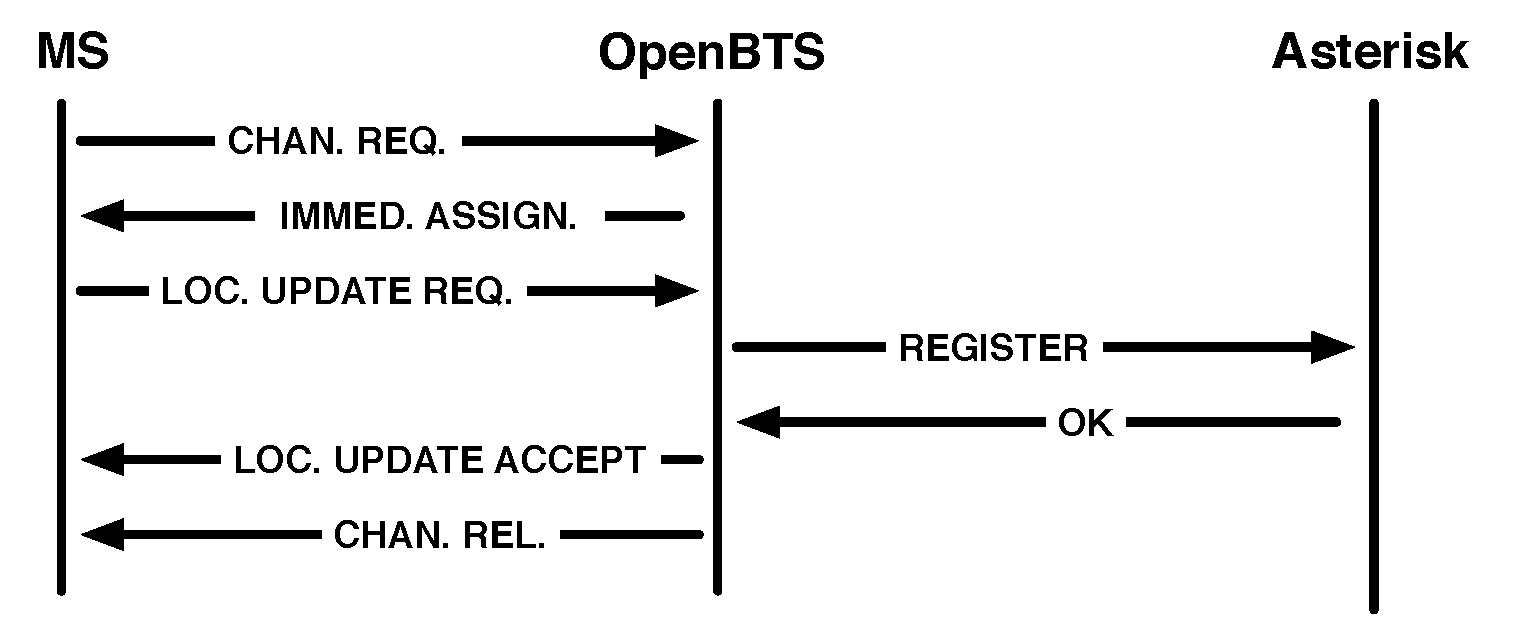
\includegraphics[width=6in]{LURLadder.pdf}
\caption{GSM location update mapped to a SIP REGISTER.}
\label{fig:LURLadder}
\end{center}
\end{figure}


\section{Call Control}
Figures \ref{fig:MTCLadder} and \ref{fig:MOCLadder} show the mobile-originated and mobile-terminated call setup cases, using very early assignment for simplicity.  In both cases, once the channel is established, the transaction ladder is essentially that of a SIP-ISDN gateway.

\begin{figure}[htbp]
\begin{center}
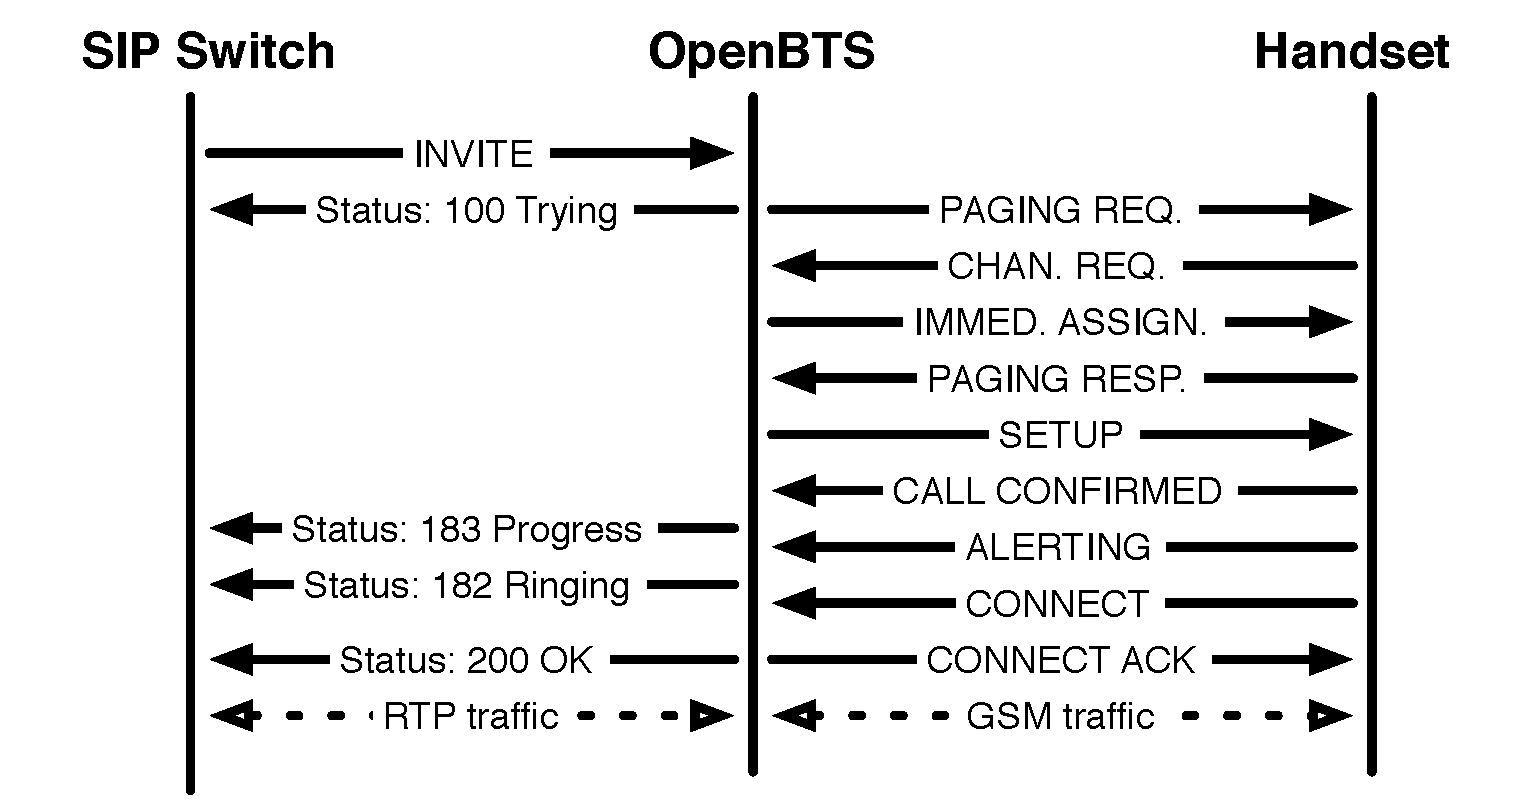
\includegraphics[width=6in]{MTCLadder.pdf}
\caption{A GSM-SIP mobile-terminated call, VEA, normal case.}
\label{fig:MTCLadder}
\end{center}
\end{figure}

\begin{figure}[htbp]
\begin{center}
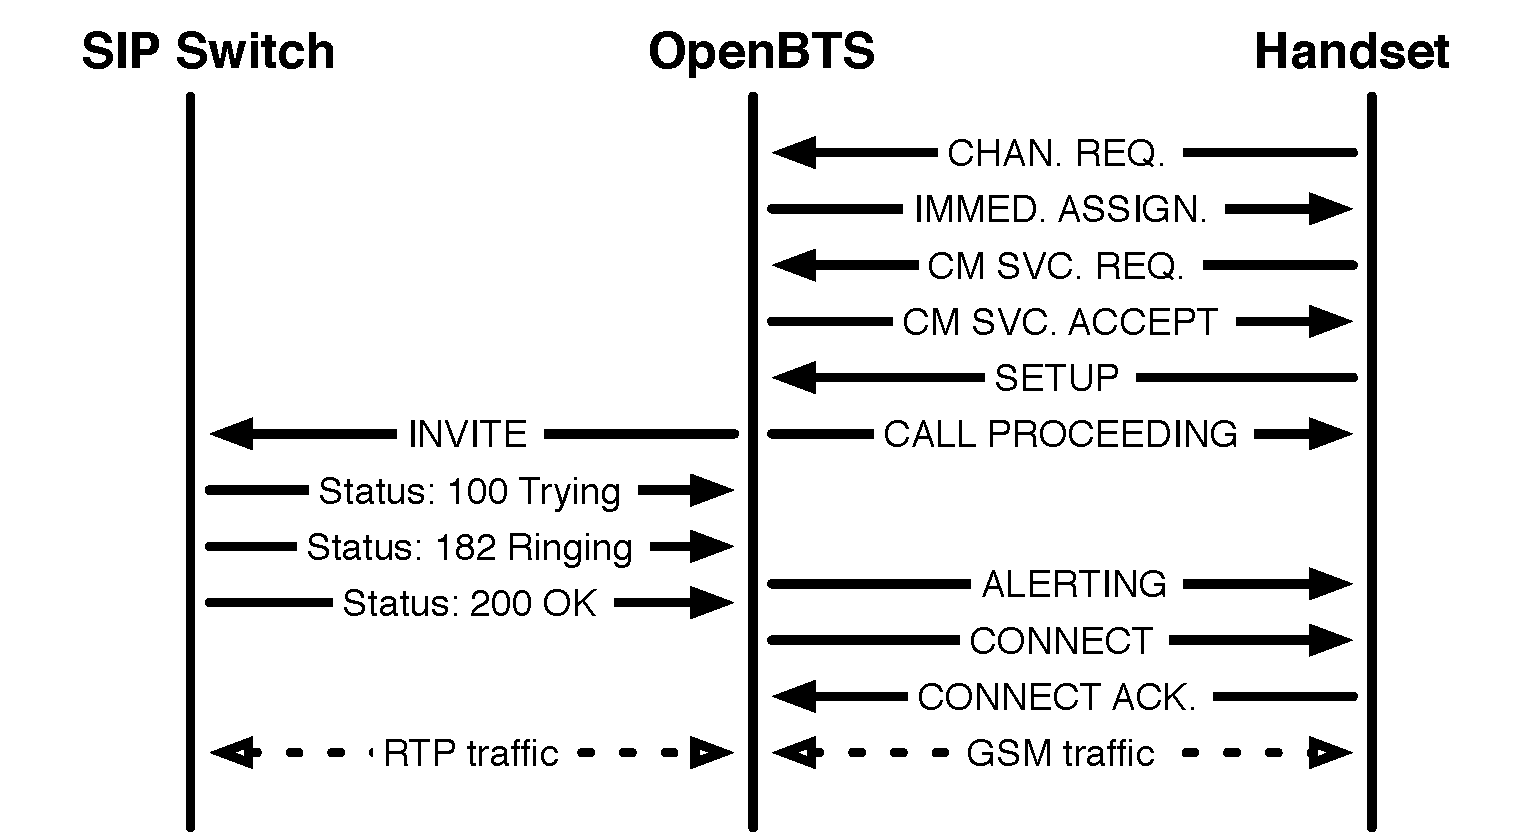
\includegraphics[width=6in]{MOCLadder.pdf}
\caption{A GSM-SIP mobile-originated call, VEA, normal case.}
\label{fig:MOCLadder}
\end{center}
\end{figure}




\chapter{Text Messaging}
\label{chap:smqueue}
GSM text messaging (``short message service'' or SMS) is a service akin to e-mail.
Users can send and receive 140-byte messages, allowing up to 160 characters using the SMS 7-bit alphabet.
Addresses can be ISDN private network, E.164 or e-mail.

\section{Internet Messaging Protocols}
For OpenBTS to handle SMS in a manner consistent with its design goals, the GSM SMS protocol must be translated to and from some open protocol from the internet world.
There are many such protocols, but few are well-suited to SMS.

\subsection{The ``Session'' Problem}
Most messaging protocols in the IETF/IP world, like XMPP, are built around the notion of a ``connected session'', a virtual circuit similar the virtual connection of RTP or TCP/IP.  This model assumes an ``always-on'' network connection where the maintenance of the circuit, with occasional keep-alive messages, is cheap and reasonable.

GSM SMS is different.  Maintaining the channel is expensive. There is no keep-alive message mechanism.  The circuit switched connection is created and destroyed with every transfer.  Each message transfer is an independent transaction.  There is no natural notion of a session.

\subsection{RFC-3428}
RFC-3428 is an IETF standard for the transfer of short messages over the internet.
Among IETF/IP protocols for messaging, RFC-3428 is special in that it supports ``page mode'' messaging, without any notion of a session.  This makes it a nature fit for SMS.  RFC-3428 is straightforward.  The sending entity sends a SIP MESSAGE method to the intended receiver.  The receiver gives one of the standard SIP responses, preferably SIP OK to indicate a successful transfer.


\section{The Smqueue Messaging Server}
The delivery of each text message depends on a store-and-forward facility in the network.
In OpenBTS, the smqueue messaging server provides this facility.
Smqueue was originally written by John Gilmore in the Summer of 2009 and was first used publicly at Burning Man 2009.
Unlike the OpenBTS application, smqueue is a GPL-only application an is not available under any other license.

\subsection{Design and Operation of Smqueue}
The core of smqueue is a table (or queue) of messages awaiting delivery.  Messages wait in this queue, potentially through multiple delivery attempts, until delivery is confirmed or until the message is determined to be undeliverable due to an unresolvable address or due to many failed delivery attempts over several hours or days.

\subsection{Addressing in Smqueue}
Smqueue recognizes two kinds of addresses: ISDN/E.164 addresses and SIP usernames.  Any all-numeric address is assumed to be and ISDN/E.164 address and smqueue will attempt to resolve it to a SIP username.  Any address that is not all-numeric is assumed to be a SIP username.

\subsection{Smqueue's Use of Asterisk}
Smqueue uses the Asterisk dialplan to resolve numeric addresses to SIP usernames (and thus to IMSIs) to determine numeric return addresses for messages submitted from handsets.  Smqueue also uses Asterisk's SIP registry to determine the IP current addresses of mobile SIP users.
This use of Asterisk requires that smqueue and Astrerisk be run on the same computer and means that the smqueue server and Asterisk server running on the same machine will always have a common IMSI-ISDN address mapping.

\subsection{Configuration of Smqueue}
Smqueue is configured through the smqueue.config file.
As of release 2.6, the configuration can be changed only be restarting smqueue after editing the file.  Some configuration parameters of note are:
\begin{itemize}
	\item Log.Level, Log.FileName -- This are logging controls that perform the same as those in OpenBTS.config.  See Section~\ref{sec:Logging} for more information.
	\item Asterisk.address -- The IP address and port number of the Asterisk server to be used for SIP registration transactions.  Normally 127.0.0.1.
	\item SIP.myIP -- The IP address of the smqueue machine as seen by the Asterisk server.  Normally 127.0.0.1.
	\item SIP.mySIP2 -- The IP address of the smqueue machine as seem by remote gateways.
	\item SIP.global\_relay -- The IP address of a remote RFC-3428 server for delivery of non-local messages.
	\item BounceMessage.* -- Error messages sent back to handsets when submitted messages are undeliverable.
	\item SC.* -- Configuration parameters for specific short code functions, not for smqueue itself.
\end{itemize}

\section{Text Messaging in GSM}
GSM 04.11 and 03.40 define conventional SMS in five layers:
\begin{enumerate}
	\item L1 is taken from the Dm channel type used, either SDCCH or SACCH. This layer terminates in the BSC.
	\item L2 is normally LAPDm. This layer terminates in the BTS.
	\item L3, the connection layer, is defined in GSM 04.11 Section 5. This layer terminates in the MSC.
	\item L4, the relay layer, is defined in GSM 04.11 Section 6. This layer terminates in the MSC.
	\item L5, the transfer layer, is defined in GSM 03.40. This layer terminates in the SMSC.
\end{enumerate}
As a general rule, every message transferred in L(n) requires both a transfer and an acknowledgment on L(n-1).

In the OpenBTS realization of SMS, there is no MSC, so L3 and L4 terminate in OpenBTS and L5 is a relay to smqueue, which takes the place of the SMSC.
The L3 and L4 parts of SMS are implemented in OpenBTS in Control/SMSControl.cpp.
The rest is in smqueue.cpp.

OpenBTS 2.6 always uses the SDCCH for SMS.  This is a simplification, but does have the effect that OpenBTS cannot transfer text messages while speech calls are in progress.

\subsection{SMS in L3}
The Um L3 part of SMS uses three messages:
\begin{itemize}
	\item CP-DATA to transfer an RPDU across Um and into L4.
	\item CP-ACK to acknowledge the transfer of an RPDU across Um and into L4.
	\item CP-ERROR to report the failure to transfer an RPDU to L4.
\end{itemize}
An RPDU is a ``relay (layer) protocol data unit'', which is just an encapsulation of a message from L4.
The operation in L3 is simple.  The entity that needs to transfer an RPDU sends it in a CP-DATA message.  The receiving entity responds with CP-ACK or CP-ERROR.  Transactions are non-overlapping.

The action of OpenBTS upon receiving CP-DATA from a handset is to verify the correct encoding of the L3 part of the message and respond with CP-ACK or CP-ERROR as appropriate.  After sending CP-DATA to a handset, OpenBTS waits for CP-ACK or CP-ERROR, proceeding after CP-ACK or aborting the transaction after CP-ERROR.


\subsection{SMS in L4}
The Um L4 part of SMS uses four messages:
\begin{itemize}
	\item RP-DATA to transfer a TPDU across Um and into L5.
	\item RP-ACK to acknowledge the transfer of a TPDU across Um and into L5.
	\item RP-ERROR to report the failure to transfer an TPDU to L5.
	\item RP-SMMA for the handset to report that it has more memory available to receive SMS messages (not supported by OpenBTS 2.6).
\end{itemize}
An TPDU is a ``transfer (layer) protocol data unit'', which is just an encapsulation of a message from L5.
The operation in L4 is simple.  The entity that needs transfer an TPDU sends it in an RP-DATA message.  The receiving entity responds with RP-ACK or RP-ERROR.  Transactions are non-overlapping.

The action of OpenBTS upon receiving RP-DATA from a handset is to attempt to rely the TPDU to smqeue and respond with RP-ACK or RP-ERROR as appropriate.  After sending RP-DATA to a handset, OpenBTS waits for RP-ACK or RP-ERROR, proceeding after RP-ACK or aborting the transaction after RP-ERROR.

\subsection{SMS in L5}
The Um L5 part of SMS, as supported by OpenBTS 2.6, uses these message:
\begin{itemize}
	\item SMS-SUBMIT to transfer a text message from the handset to the network.
	\item SMS-DELIVER to transfer a text message from the network to the handset.
\end{itemize}

Upon receiving SMS-SUBMIT from a handset, OpenBTS translates the TPDU into a corresponding RFC-3428 SIP message and sends it to smqueue.  When smqueue responds with SIP OK, OpenBTS sends RP-ACK to the handset.  If this operation times out, OpenBTS responds to the handset with RP-ERROR.

When OpenBTS receives an RFC-3824 message from smqueue for a handset, it translates that message to an SMS-DELIVER, sends it to the handset and waits for RP-ACK or RP-ERROR.  When OpenBTS receives RP-ACK, it produces a SIP OK reply to smqueue.  Upon receiving RP-ERROR, OpenBTS simply aborts the GSM transaction and closes the radio channel.


\subsection{RFC-3428 and SMS in OpenBTS}
Now we take a look at all of the GSM layers and the SIP transactions together.

\subsubsection{Mobile Terminated}

Figure~\ref{fig:MTSMSLadder} shows a complete mobile terminated SMS transfer, where the network, through smqueue, transfers a text message to the handset.  The message arrives at smqueue from the outside world addresses either to a SIP user or to a numeric address.  Smqueue resolves the destination address to an IMSI and forwards the message to OpenBTS.  OpenBTS pages the handset, establishes a channel, transfers the message as SMS and then responds to smqueue with OK.

The most common failure in the mobile terminated transfer is that the handset does not respond to paging.  In this case, smqueue never receives any response.  The message remains in the smqeue delivery queue and another delivery attempt will be made in a few minutes.

\begin{figure}[htbp]
\begin{center}
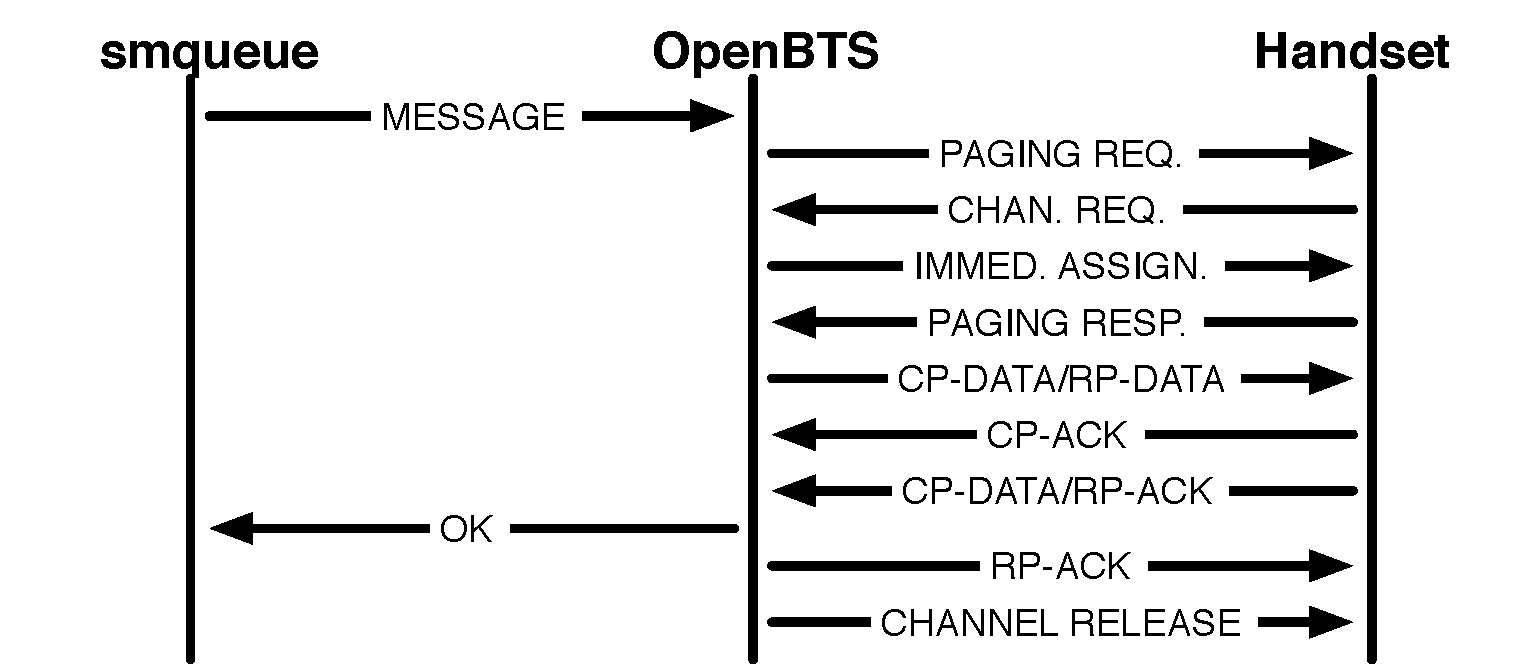
\includegraphics[width=6in]{MTSMSLadder.pdf}
\caption{Mobile-terminated SMS transfer, normal case.}
\label{fig:MTSMSLadder}
\end{center}
\end{figure}

\subsubsection{Mobile Originated}

Figure~\ref{fig:MOSMSLadder} shows a complete mobile originated SMS transfer, where the handset, transfers a text message to smqueue for later delivery to its addressee.  The message originates in the handset with a numeric address.  The handset establishes a radio channel to OpenBTS and then sends the text message TPDU in an RP-DATA message.  OpenBTS translates the TPDU to a SIP MESSAGE method and sends that to smqueue.  Smqueue responds with OK and then OpenBTS responds to the handset with RP-ACK.

\begin{figure}[htbp]
\begin{center}
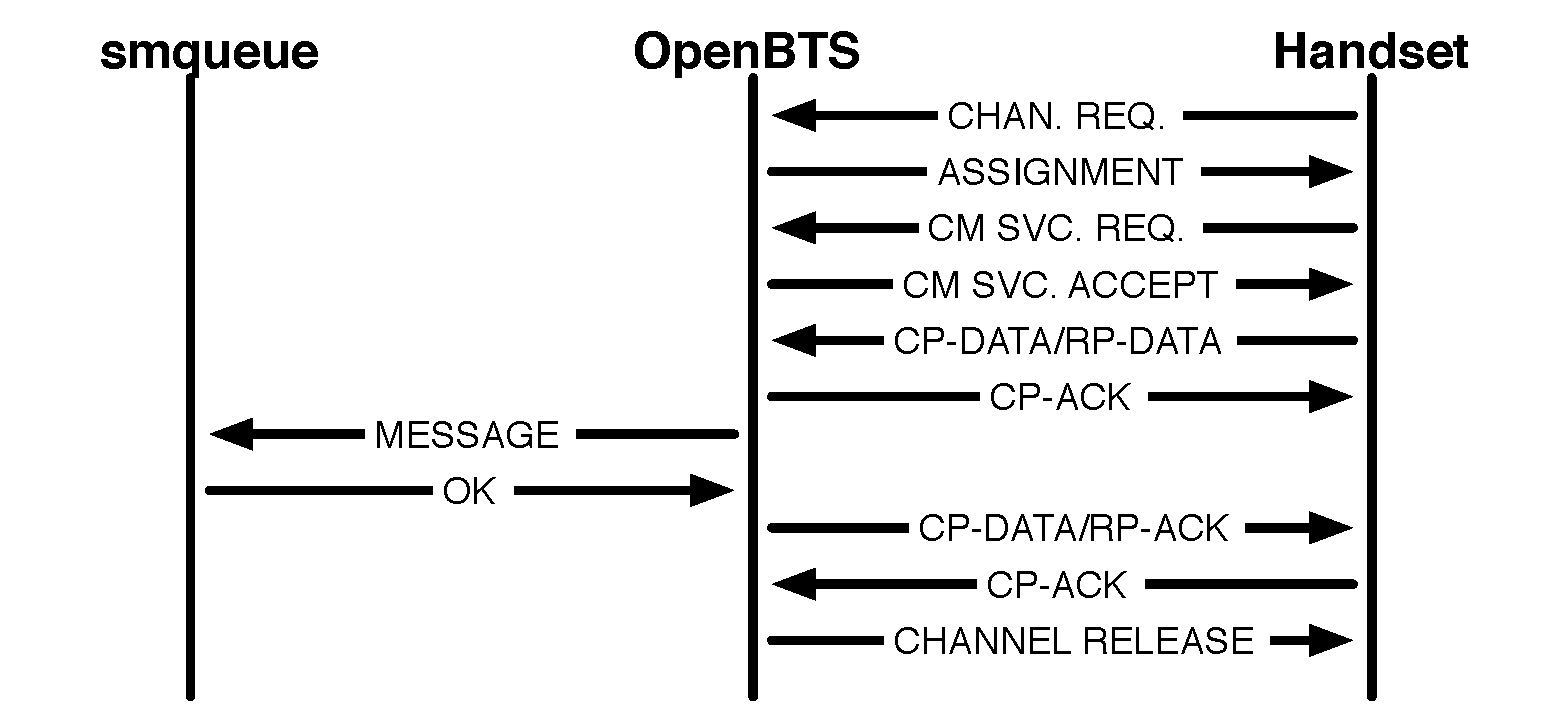
\includegraphics[width=6in]{MOSMSLadder.pdf}
\caption{Mobile-originated SMS transfer, normal case.}
\label{fig:MOSMSLadder}
\end{center}
\end{figure}


\section{Short Code Applications}
Short codes are local addresses within smqueue that terminate in local application code.  A message sent to a short code becomes an input argument to a short code handler function, instead of being delivered to another user. Short code functions provide a means of writing interactive applications based on text messaging.
A typical SMS-based application would normal comprise several short code addresses and handlers sharing common data.

\subsection{Short Code Implementation}
The short code implementation in OpenBTS 2.6 is primitive but functional.  Each short code handler is a C++ function coded directly into smqueue/smcommands.cpp.  The arguments to a short code handler are the source IMSI of the message, the message text and a short\_code\_params data structure into which any reply message can be written.  The return value from a short code handler is a status code called short\_code\_action.  See smqueue/smcommands.cpp for examples.

Once a short code handler function is defined, it must also be registered at an address.  This happens in SMqueue::init\_smcommands(), also defined in smqueue/smcommands.cpp.

\subsection{Existing Short Code Applications}
There are a few interesting short code applications built in to the standard release of smqueue, although they are all simple applications each requiring only a single handler function.

\subsubsection{Autoprovisioning (``Register'')}
\label{sec:autoprovisioning}
The autoprovisioning application allows OpenBTS users to create new entries in the Asterisk SIP configuration and dialplan via SMS.  The user sends his desired telephone number in a text message to the autoprovisioning short code address.  If the requested number has an acceptable number of digits and is not already assigned to a user, the autoprovisioning handler function will perform the steps described in Section~\ref{sec:provisioning} to provision the new user into the Asterisk server in the sip-local context.  The autoprovisioning short code handler function is called shortcode\_register and it is configured through the SC.Register.* parameters in smqueue.config.

For autoprovisioning to work, you must enable the open registration feature, so that unprovisioned handsets will show service and be capable of sending text messages.  The open registration welcome message can be a powerful way to advertise this feature, especially if the return short code of the welcome message is the same as the short code of the autoprovisioning function.  See Sections~\ref{sec:openReg} and \ref{sec:welcomeMessages} for more information.

\subsubsection{Whiplash Quit}
The whiplash\_quit shortcode handler shuts down smqueue is the correct passphrase is sent to the correct address.  This function is useful for development, but should be disabled in deployed systems.   This short code handler can be configured with the  SC.WhiplashQuit.* parameters in smqueue.config.
To disable it, comment out SC.WhiplashQuit.Code in smqueue.config.

\subsubsection{Info}
This short code handler generates a brief report of smqueue status, returned in a text message.  The implementing function is called shortcode\_four\_one\_one. This short code handler can be configured with the  SC.Info.* parameters in smqueue.config.

\subsubsection{Zap Queued}
The shortcode\_zap\_queued handler can delete a message with a specific hash tag or can delete all messages in the queue older than 5000 seconds.  This short code handler can be configured with the  SC.ZapQueued.* parameters in smqueue.config.


\chapter{Mobility}
``Mobility'' is the ability to transfer a handset's service as it moves from one BTS unit to another in a multi-BTS network so that inbound calls for that handset get routed to it correctly.  Mobility is one of the defining features of a cellular network.  Although OpenBTS 2.6 does not support the transfer of a live call between BTS units, it does support mobility.  A handset can move through a multi-BTS network and inbound calls and text messages will be routed to it correctly. In this chapter, we will consider the simplest OpenBTS 2.6 mobility implementation, where multiple BTS units share a common Asterisk/smqueue server machine.  An example of such a network is shown in Figure~\ref{fig:NetworkArch}, where four BTS units share a common Asterisk/smqueue server machine.

\begin{figure}[htbp]
\begin{center}
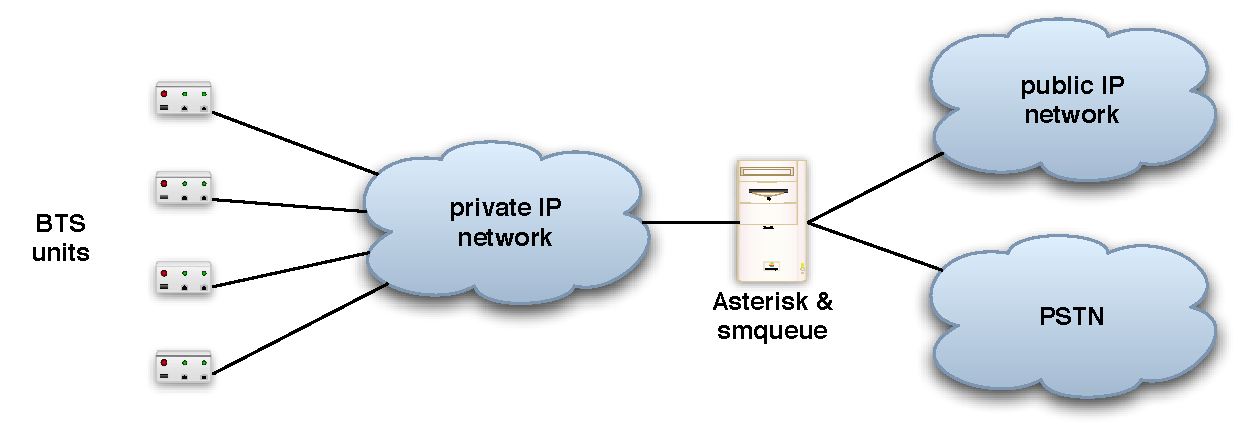
\includegraphics[width=6in]{NetworkArch.pdf}
\caption{A four-BTS network with a common server.}
\label{fig:NetworkArch}
\end{center}
\end{figure}


\section{How Mobility Works in GSM}
There are two mobility mechanisms in GSM that are implemented in OpenBTS: the location area and the neighbor list.

\subsection{Location Areas}
A GSM network is divided into geographical regions called ``location areas'', each one typically served by a single BSC.  Every BTS broadcasts its location area code (LAC) on the BCCH.  In OpenBTS~2.6, the LAC is controlled with the GSM.LAC configuration parameter, which is dynamic and can be altered in real time.  A handset performs a location updating request whenever it enters a new location area.  When a handset is paged for an inbound call, the paging request is sent to all of the cells in the location area in which a handset is registered.  The implication here is that the GSM core network does not need to know the specific cell that is serving a handset, only its location area.  However, if every cell in the network has a different LAC, the handset will perform a location updating request every time it moves to a new cell.

\subsection{Neighbor Lists}
Every BTS broadcasts a list of ARFCNs of neighboring cells, called the neighbor list, on the BCCH.  This list is also sent on the SACCH during transactions and calls.  The handset monitors these ARFCNs, measuring their power levels and decoding their SCH bursts.  In idle mode, the handset compares these power levels to the power level of its serving cell. When the power level of the strongest neighbor exceeds that of the serving cell by a given threshold, the handset will recamp from the current serving cell to the strong neighbor.  The power threshold at which this happens is called the ``cell reselection hysteresis'', a parameter broadcast on the BCCH.  If the new cell has a different LAC that the previous cell, the handset will also make a location updating request to insure proper routing of inbound calls.

\subsection{BTS Configuration}
In the OpenBTS~2.6 configuration, the following parameters are relevant:
\begin{itemize}
	\item GSM.ARFCN -- The operating ARFCN (static).
	\item GSM.NCC -- The network color code, a 3-bit value used by all of the cells in a given network (dynamic).
	\item GSM.BCC -- The basestation color code, a 3-bit value that should be different from those on the neighboring BTS units.
	\item GSM.Neighbors -- The neighbor list (dynamic).
	\item GSM.CS.CELL\_RESELECT\_HYSTERESIS -- The idle mode cell reselection hysteresis (dymanic). See GSM 04.08 Section 10.5.2.4 for information about the encoding of this parameter.
	\item GSM.CS.NCCsPermitted -- A mask of NCCs to be monitored by the handset (dynamic, also sent on the BCCH).  Be sure your own NCC is set in this mask!
\end{itemize}

\section{How Mobility Works in SIP}
From the point of view of Asterisk, a mobile SIP user is a user whose IP address changes.  Asterisk supports this with the ``host=dynamic'' qualifier in the SIP user profile.  In the SIP registry, Asterisk keeps track of the IP address from which a user last registered.  (These IP addresses can be observed from the Asterisk console with the ``sip show peers'' command.)  Once a user is registered to a given IP address, all inbound calls for that user are routed to that address.

\section{Combined GSM-SIP Mobility in OpenBTS}
OpenBTS translates every GSM location updating operation into a SIP registration transaction, as explained in Section~\ref{sec:GSMLUR}.  The handset performs a location update every time it moves into a new location area. So if we give every BTS a different LAC the handset will perform a location update every time it camps to a new cell, resulting in a SIP registration that updates the handset's associated IP address in Asterisk's SIP registry.  Because smqueue also uses the Asterisk SIP registry for address resolution and message routing, SMS routing will be updated as well.

Note that this mobility approach does not require the Asterisk and smqueue servers to have any prior knowledge of the BTS units.  New BTS units can be added to and removed without any modifications to the core network.

\subsection{Example OpenBTS Configuration}
In this example configuration, there is a central Asterisk/smqueue server in a private IP network at 192.168.1.20.  There are three BTS units in the same subnet and the allowed ARFCNs are 40, 42, and 44.  For simplicity, we show only the configuration parameters related to mobility.

For BTS unit A, on ARFCN 40 at IP 192.168.1.30:
\begin{verbatim}
Asterisk.IP 192.168.1.20
Smqeue.IP 192.168.1.20
SIP.IP 192.168.1.30
GSM.ARFCN 40
GSM.Neighbors 42 44
GSM.NCC 0
GSM.BCC 0
GSM.LAC 1000
GSM.CS.NCCsPermitted 1
GSM.CS.CELL_RESELECT_HYSTERESIS 3
\end{verbatim}

For BTS unit B, on ARFCN 42 at IP 192.168.1.31:
\begin{verbatim}
Asterisk.IP 192.168.1.20
Smqeue.IP 192.168.1.20
SIP.IP 192.168.1.31
GSM.ARFCN 42
GSM.Neighbors 40 44
GSM.NCC 0
GSM.BCC 1
GSM.LAC 1001
GSM.CS.NCCsPermitted 1
GSM.CS.CELL_RESELECT_HYSTERESIS 3
\end{verbatim}

For BTS unit C, on ARFCN 44 at IP 192.168.1.32:
\begin{verbatim}
Asterisk.IP 192.168.1.20
Smqeue.IP 192.168.1.20
SIP.IP 192.168.1.32
GSM.ARFCN 44
GSM.Neighbors 40 42
GSM.NCC 0
GSM.BCC 2
GSM.LAC 1002
GSM.CS.NCCsPermitted 1
GSM.CS.CELL_RESELECT_HYSTERESIS 3
\end{verbatim}

Note the following about the configurations:
\begin{itemize}
	\item Asterisk.IP and Smqueue.IP are the same everywhere, pointing all of the BTS units to a common server.
	\item SIP.IP is the IP address of each BTS as seen by the Asterisk server.
	\item GSM.ARFCN is different on each BTS.
	\item GSM.Neighbors lists all of the \emph{other} BTS ARFCNs on each BTS.
	\item GSM.NCC is the same on all units.
	\item GSM.BCC is different on all units.
	\item GSM.LAC is different on all units.
	\item GSM.CS.NCCsPermitted is 1 because GSM.NCC is 0, so the NCC mask selects just the NCC for this network.
	\item GSM.CS.CELL\_RESELECT\_HYSTERESIS is 3, giving a hysteresis of 6~dB, so whenever a neighboring cell is measured to be more than 6~dB stronger than the serving cell, the handset will recamp to the neighbor, which will trigger a registration in the Asterisk server at the new cell's IP address.
\end{itemize}
 \end{document}

 